\documentclass[11pt,a4paper]{book}

%------- packges ---------_%
% author's contact footnote
\usepackage{authblk}
\usepackage[right=1.25in,left=1.25in,top=1.1in,bottom=1.1in]{geometry}
% math tools
\usepackage{amsmath}
\usepackage{amsfonts}
\usepackage{amssymb}
\usepackage{amsthm}
\usepackage{mathtools}
\usepackage{mathrsfs}
% making hyperlinks blue
\usepackage[hidelinks]{hyperref}
\usepackage{xcolor}
\hypersetup{
	colorlinks,
	linkcolor={red!50!black},
	citecolor={blue!50!black},
	urlcolor={blue!80!black}
}
%bib also backref and blue
\usepackage{enotez}
\setenotez{backref}
\usepackage{float}
%enable footnotes' brackets
%\renewcommand*{\thefootnote}{(\arabic{footnote})}
%\renewcommand*{\theendnote}{(\arabic{endnote})}
%enable to collect footnotes as endnote
%\let\footnote = \endnote

%\usepackage{float}
\usepackage{ulem}
% creating nice table (\toprule, \midrule, \bottomrule)
\usepackage{booktabs}
\usepackage{threeparttable}

%make enumerate alphabetical instead of bullets
\usepackage{enumitem}
%\begin{enumerate}[label=(\alph*)] to use a), b), c) \end{enumerate}
%\begin{enumerate}[label=(\roman*)] \end{enumerate} to use i), ii), iii)

% tikz
\usepackage{tikz}
\usepackage{tikzscale}
\usetikzlibrary{arrows,calc, automata, patterns, positioning, shapes.geometric, decorations.pathreplacing,decorations.markings}

%to insert images side-by-side, change fig names
\usepackage[font=small,labelfont=bf,
justification=justified,
format=plain]{caption}
\captionsetup[figure]{name=Fig. ,labelsep=period}
\usepackage{subcaption}
\usepackage{graphicx}
\usepackage{rotating}


%----------bib manager---------%
%\usepackage[backend=bibtex,style=authoryear,natbib=true]{biblatex} 
\usepackage{natbib}
\bibliographystyle{apalike}
% Use the bibtex backend with the authoryear citation style (which resembles APA)
%to cite normally, use \textcite{}, and to cite with parentheses, use \parencite{}
\usepackage[autostyle=true]{csquotes} % Required to generate language-dependent quotes in the bibliography
%--offline
%\addbibresource{bibliography.bib} 
%--online
%\addbibresource[location=remote]{biblink}

%add plot
\usepackage{pgfplots}
\usepgfplotslibrary{groupplots}
\pgfplotsset{width=10cm,compat=1.9}

% color scheme
\newcommand{\red}[1]{\textcolor{red}{#1}}
\newcommand{\blue}[1]{\textcolor{blue}{#1}}
\newcommand{\green}[1]{\textcolor{green}{#1}}
\newcommand{\teal}[1]{\textcolor{teal}{#1}}

% quick maths
\newtheorem{theorem}{Theorem}[section]
\newtheorem{corollary}{Corollary}[theorem]
\newtheorem{lemma}[theorem]{Lemma}
\newtheorem{assumption}{Assumption}
\theoremstyle{definition}\newtheorem{definition}{Definition}
\newtheorem{prop}{Proposition}
\newtheorem{notation}{Notation}
\theoremstyle{definition}\newtheorem{fact}{Fact}
\theoremstyle{definition}\newtheorem{remark}{Remark}
\renewcommand\qedsymbol{$\blacksquare$}
\theoremstyle{definition}\newtheorem{ex}{Ex.}
\theoremstyle{definition}\newtheorem{project}{Project}
%problem/solution env

\theoremstyle{definition}\newtheorem{problem}{Problem}
\newenvironment{solution}{\begin{proof}[Solution]}{\end{proof}}
\theoremstyle{definition}\newtheorem{example}{Example}


%add frame for important stuff
\usepackage{mdframed}
\newenvironment{ftheorem}
{\begin{mdframed}\begin{theorem}}
		{\end{theorem}\end{mdframed}}
\newenvironment{fdefinition}
{\begin{mdframed}\begin{definition}}
		{\end{definition}\end{mdframed}}
\newenvironment{fprop}
{\begin{mdframed}\begin{prop}}
		{\end{prop}\end{mdframed}}
\newenvironment{fnotation}
{\begin{mdframed}\begin{notation}}
		{\end{notation}\end{mdframed}}

% numbering
\numberwithin{theorem}{section}
\numberwithin{corollary}{chapter}
\numberwithin{assumption}{chapter}
\numberwithin{definition}{chapter}
\numberwithin{prop}{chapter}
\numberwithin{notation}{chapter}
\numberwithin{problem}{chapter}
\numberwithin{example}{chapter}
\numberwithin{fact}{chapter}
\numberwithin{ex}{chapter}


%--- to insert plain text---
%\texttt{code}

%convenience
%mathbb
\def\R{\mathbb R}
\def\N{\mathbb N}
\def\E{\mathbb E}
\def\P{\mathbb P}

%mathcal
\def\cP{\mathcal P}
\def\cS{\mathcal S}
\def\cX{\mathcal X}
\def\cY{\mathcal Y}
\def\cA{\mathcal A}
\def\cB{\mathcal B}
\def\cW{\mathcal W}

%mathbf
\def\1{\mathbf 1}
\def\0{\mathbf 0}
\def\A{\mathbf A}
\def\B{\mathbf B}
\def\C{\mathbf C}
\def\D{\mathbf D}
\def\E{\mathbf E}
\def\M{\mathbf M}
\def\N{\mathbb N}
\def\O{\mathbf O}
\def\P{\mathbf P}
\def\Q{\mathbf Q}
\def\R{\mathbb R}
\def\S{\mathbf S}
\def\I{\mathbf I}
\def\J{\mathbf J}
\def\T{\mathbf T}
\def\a{\mathbf a}
\def\b{\mathbf b}
\def\c{\mathbf c}
\def\e{\mathbf e}
\def\F{\mathbf F}
\def\G{\mathbf G}
\def\H{\mathbf H}
\def\h{\mathbf h}
\def\g{\mathbf g}
\def\m{\mathbf m}
\def\p{\mathbf p}
\def\q{\mathbf q}
\def\r{\mathbf r}
\def\s{\mathbf s}
\def\t{\mathbf t}
\def\u{\mathbf u}
\def\v{\mathbf v}
\def\U{\mathbf U}
\def\w{\mathbf w}
\def\x{\mathbf x}
\def\y{\mathbf y}
\def\Y{\mathbf Y}
\def\z{\mathbf z}
\def\Z{\mathbb Z}
\def\X{\mathbf X}

% appendix appears in toc
\usepackage[titletoc]{appendix}



% ENUMERATE
\usepackage{enumitem}
% [label=(\alph*)] 
% [label=(\Alph*)]
%[label=(\roman*)]

%AUTHOR FOOTNOTE



%=================================================%
%										 FRONT MATTER 
%=================================================%


\author{%
	TRAN Quang-Thanh (Tedd) \thanks{tran.quang.thanh.p1@dc.tohoku.ac.jp}
	
	\and ZHANG Ye (Tony)  \thanks{zhang.ye.q8@dc.tohoku.ac.jp} 
		}

\title{INSEIKAI Tohoku Summer Camp 2023 \\ \textbf{Mathematics II: Dynamic Optimization, Financial Mathematics and Economic Modeling}}

\date{Graduate School of Economics and Management \\Tohoku University \\[\baselineskip] \today}


%=================================================%
%										 MAIN 
%=================================================%


\begin{document}
	{
		\makeatletter
		\addtocounter{footnote}{1} % to get dagger instead of star
		\renewcommand\thefootnote{\@fnsymbol\c@footnote}%
		\makeatother
		\maketitle
	}
	
	\setcounter{footnote}{0}
	\setcounter{tocdepth}{3}
	\tableofcontents
	
	\chapter{Difference Equations}
	In economic growth theory, in studies of the extraction of natural resources, in many models in environmental economics, and in several other areas of economics that have one key variable moves based on its past values, you will have to deal with dynamics. If we talk about dynamics, we talk about difference (in discrete time), or differential (in continuous time) equations. For the scope of this course, we are only concerned about the first-order difference equation, that is, tomorrow's value only depends on today, not including yesterday. All the materials presented here are from \citet{sydsaeter2008essential, sydsaeter2008further} and \citet[p.616]{chiang1984fundamental}. For differential equations, read \citet[Chapter 5, 6]{sydsaeter2008further}, \citet[Chapter 23,24,25]{simon1994mathematics}
	
	%=================================================%
	%										 CHAP 1
	%=================================================%
	
	%\section{Difference Equations}
	\section{One Variable: Linear case}
	A simple example of a linear first-order difference equation is
	\begin{align*}
		x_{t+1} = a x_t
	\end{align*}
	for $t = 0.1,\dots$ and $a$ is a constant. Suppose $x_0$ is given, if we repeatedly applying the function for different $t$, we get
	\begin{align*}
		x_1 &= a x_0, \\
		x_2 &= a x_1 = a^2 x_0, \\
		x_3 &= a x_2 = a^3 x_0, \dots
	\end{align*}
	which we can generalize it as
	\begin{align*}
		x_t = x_0 a^t
	\end{align*}
	So that at any time $t$, given $a_0$ is known, we can calculate the current value of $x_t$. We can expand it by adding a constant $b$\footnote{If $b = g(t)$, that is, the difference equation also depends on time $t$, then it is called non-autonomous. If the difference equation does not depend on $t$, then it is called autonomous}. so the difference equation becomes
		\begin{align}
			x_{t+1} = a x_t + b \label{diff1}
	\end{align}
	which gives us
	\begin{align*}
		x_t = a^t \left(x_0 - \frac{b}{1-a} \right) + \frac{b}{1-a} && (a \neq 1 )
	\end{align*}
	We now discuss the notion of \textbf{stationary point}. Consider the solution of \eqref{diff1}. If
	\begin{align*}
		x_0 = \frac{b}{1-a}
	\end{align*}
	then 
	\begin{align*}
		x_t = \frac{b}{1-a} \ \forall t
	\end{align*}
	This solution $\bar{x} = b/(1-a)$ is called an equilibrium, or stationary, or steady state of \eqref{diff1}. To find such an equilibrium state $\bar{x}$, we need to find $\bar{x}$ such that
	\begin{align*}
		\bar{x} = a \bar{x} + b
	\end{align*}
	Suppose that $|a| < 1$ then 
	\begin{align*}
		\lim_{t\to \infty} a^t = 0
	\end{align*}
	implying that
	\begin{align*}
		\lim_{t \to \infty} x_t = \frac{b}{1-a}
	\end{align*}
	Hence, so long as $-1 < a < 1$, the solution converges to the equilibrium state as $t\to \infty$ and we say that the difference equation is globally asymptotically stable. But would happen otherwise?
	
	Let us now discuss \textbf{stability} by the following illustration.
	\begin{figure}[H]
		\centering
		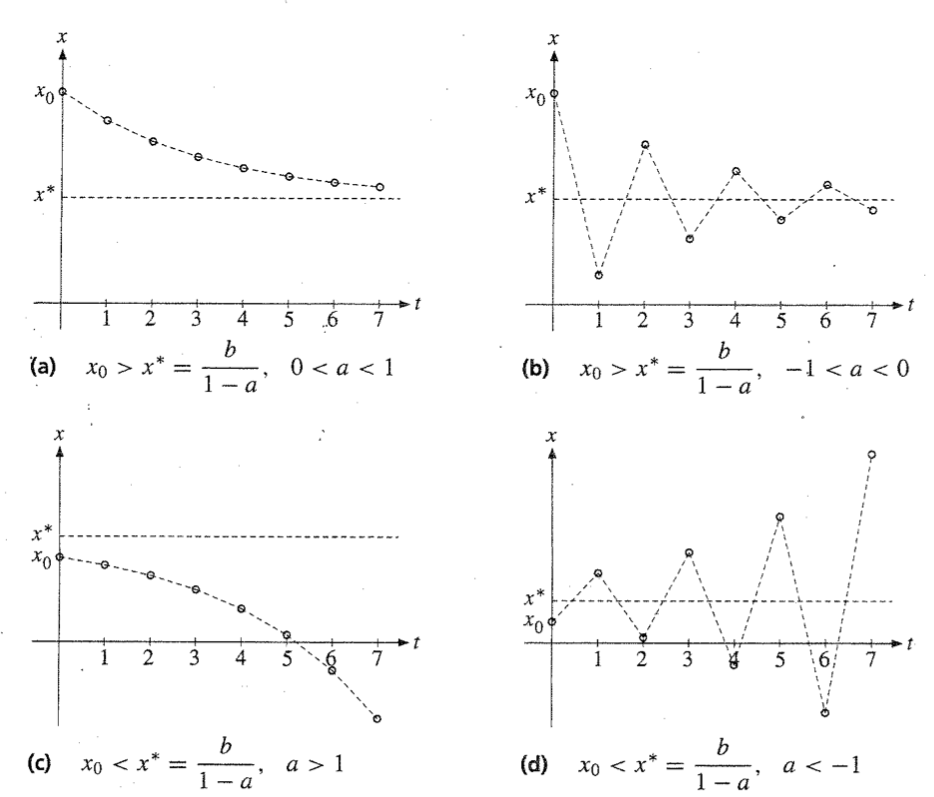
\includegraphics[scale=0.35]{figs/page393.png}
		\caption{Dynamics of stable and unstable equations \citep[p.393]{sydsaeter2008further} } 
		\label{fig:stablity}
	\end{figure}
	
	We summarize the cases in Fig.\ref{fig:stablity} as follows.
	\begin{enumerate}[label=(\alph*)]
		\item $x_t$ decreases monotonically and converges to the equilibrium state $x^*$.
		\item $x_t$ exhibits decreasing fluctuations, or \textbf{damped oscillations} around $x^*$.
		\item $x_t$ tends to $-\infty$ monotonically (it never reaches $x^*$).
		\item $x_t$ exhibits increasing fluctuations, or \textbf{explosive oscillations} around $x^*$. It does cross $x^*$ at some point but never converges to it.
	\end{enumerate}
	Thus, the condition that $|a| < 1$ is necessary to guarantee that the dynamics of $x_t$ converge to the steady state $x^*$.
	
	\section{One Variable: Nonlinear case}
	So far, we only consider linear difference equations. Although this case is easy, we almost never encounter them in economics because most dynamics in economics are nonlinear. Let us consider an autonomous first-order difference equation of one variable
	\begin{align}
		x_{t+1} = f(x_t) \label{nonlin}
	\end{align}
	The procedure to find the stationary point is still the same. We still need to solve for $\bar{x}$ such that
	\begin{align*}
		\bar{x} = f(\bar{x})
	\end{align*}
	The solution to this is called a fixed point. How can we determine the stability of this fixed point? 
	
	\begin{figure}[ht]
		\centering
		\begin{subfigure}[b]{0.63\textwidth}
			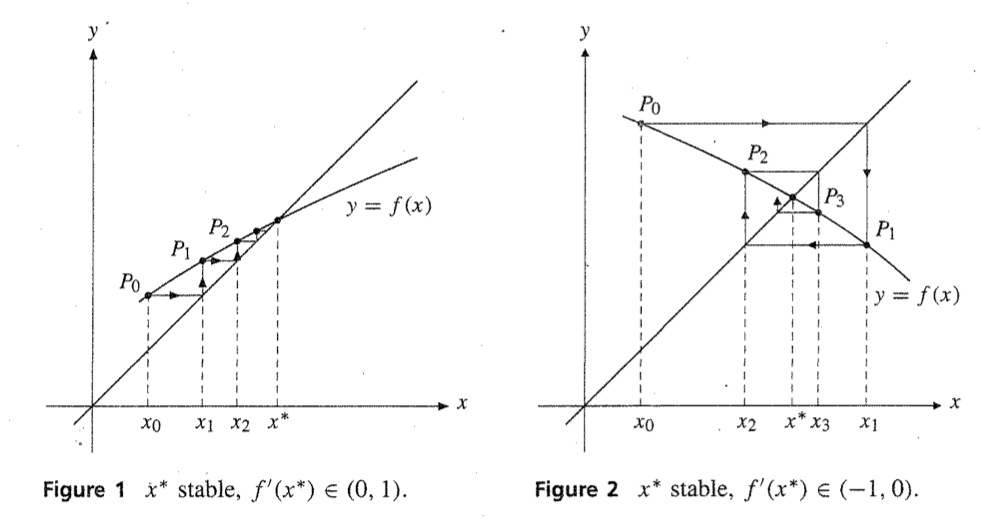
\includegraphics[width=1\linewidth]{figs/page417_1.png}
			\caption{Stable $f'(x_t) < 1$ }
			\label{fig:Ng1} 
		\end{subfigure}
		\begin{subfigure}[b]{0.63\textwidth}
			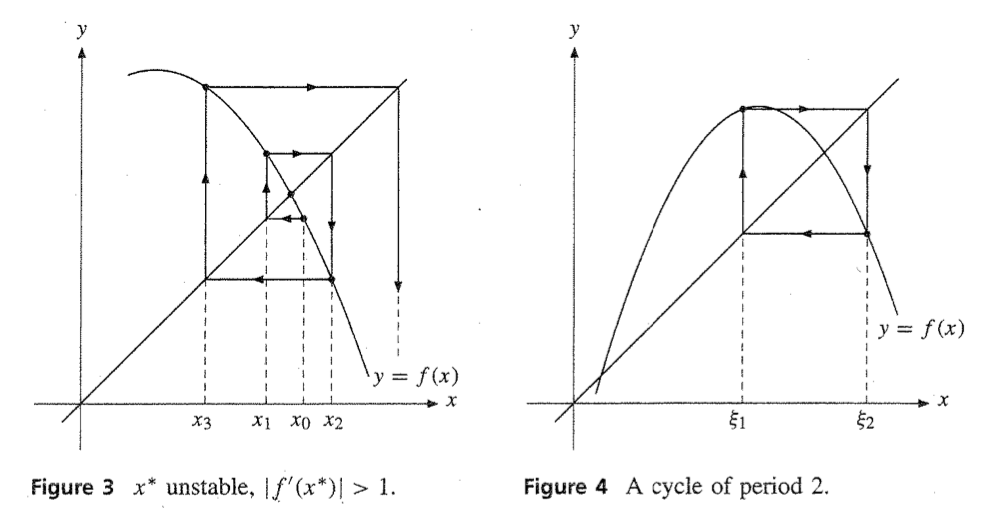
\includegraphics[width=1\linewidth]{figs/page417_2.png}
			\caption{Unstable $f'(x_t) > 1$}
			\label{fig:Ng2}
		\end{subfigure}
		\caption{Dynamics of some nonlinear equations \citep[p.420]{sydsaeter2008further}}
		\label{fig:diff2}
	\end{figure}
	
	\begin{ftheorem}[Stability condition] \label{theorem:stability}
		Let $\bar{x}$ be a stationary state for the difference equation $x_{t+1} = f(x_t)$, and suppose that $f$ is differentiable in an open interval around $x^*$.
		\begin{enumerate}
			\item If $|f'(x^*)| < 1$, then $x^*$ is \textbf{locally asymptotically stable}
			\item If $|f'(x^*)| > 1$, then $x^*$ is \textbf{unstable}
		\end{enumerate}
	\end{ftheorem}
	For the proof, see \citet[p.419]{sydsaeter2008further}
	
	Again, let us examine the stability illustrated in Fig.\ref{fig:diff2}. 
	\begin{enumerate}
		\item Here, $0< f'(x^*) < 1$ (derivative is positive) so the sequence monotonically converges to $x^*$.
		\item In this case, $-1 < f'(x^*) < 0$ (derivative is negative) so $x_t$ alternates between values above and below the equilibrium state $x^*$. Eventually, it will converge to $x^*$.
		\item This is the first case of unstable dynamics. Since $f'(x^*) > 1$, $x$ is getting farther away from the equilibrium point.
		\item This is a special case where solutions exhibit cyclic behavior (in this case, a cycle of period 2).
	\end{enumerate}
	
	Let us explore the last case in more detail. A cycle of period 2 has the following property
	\begin{align*}
			\text{first cycle} && x_0 &= x_2 = x_4 = \dots, \\
			\text{second cycle} &&x_1 &= x_3 = x_5 = \dots, \\
			\text{the 2 cylces are different} && x_0 &\neq x_1
	\end{align*}
	This case happens if and only if there are 2 solutions for  \eqref{nonlin}. Let us call them $\xi_1, \xi_2$. (pronounced /ksai/ or /zai/). Hence
	\begin{align*}
		\xi_1 = f(\xi_1), \\
		\xi_2 = f(\xi_2). 
	\end{align*}
	If we let $F = f \circ f$, it is clear that $\xi_1$ and $\xi_2$ must be fixed points of $F$ and hence the equilibria of the difference equation
	\begin{align*}
		y_{t+1} = F(y_t) = f(f(y_t)),
	\end{align*}
	where $y_t = x_t x_{t+1}$. Now, we change the focus only to the stability of $y_t$. Applying Theorem \ref{theorem:stability}, the dynamic is stable if and only if $F'(y_t) < 1$. By Chain rule
	\begin{align*}
		F'(x) = f' ( f(x) ) \cdot f'(x)
	\end{align*}
	so that
	\begin{align*}
		F'(\xi_1) = f' ( f(\xi_2) ) f'(\xi_1) = f'(\xi_2) f'(\xi_1)  = F'(\xi_2).
	\end{align*}
	Therefore, we can state 
	\begin{theorem}
		If \eqref{nonlin} admits a cycle of period 2, alternating between values $\xi_1$ and $\xi_2$, then:
		\begin{enumerate}
			\item If $| f'(\xi_1) f'(\xi_2) | < 1$, the cycle is locally asymptotically stable.
			\item If $| f'(\xi_1) f'(\xi_2) | > 1$, the cycle is unstable.
		\end{enumerate}
	\end{theorem}
	
	\section{System of 2 Difference Equations}
	Things get more complicated when there are 2 variables revolving around each other. Consider the following case system
	\begin{align}
		\begin{matrix}
			x_{t+1} = f (x_t, y_t) \\
			y_{t+1} = g (x_t, y_t)
		\end{matrix} \label{sys_nonlin}
	\end{align}
	Functions $\phi, \psi$ can be linear or nonlinear, just like the case with one variable. Before diving into things, let us take a detour and do some exercises on finding the eigenvalues of a matrix.
	
	\subsection{Eigenvalues}
	\textbf{Definition:}
	Given a square matrix $\A$, an eigenvalue of $\A$ is a scalar $\lambda$ for which there exists a non-zero vector $v$ such that the following equation holds:
	\[ \A v = \lambda v \]
	
	Here, $v$ is called an eigenvector corresponding to the eigenvalue $\lambda$. In other words, when the matrix $\A$ is applied to the vector $v$, the resulting vector is a scalar multiple of $v$ (scaled by $\lambda$). \footnote{To understand more intuitively, visit: \url{https://www.youtube.com/watch?v=PFDu9oVAE-g&list=PL0-GT3co4r2y2YErbmuJw2L5tW4Ew2O5B&index=14} }
	
	\textbf{Steps in finding the Eigenvectors and Eigenvalues}
	\begin{align*}
		\A \x = \lambda \x                   \\
		\Rightarrow (\A - \lambda) \x = 0    \\
		\Rightarrow (\A - \lambda \I) \x = 0 \\
		\iff \det (\A - \lambda \I) = 0      
	\end{align*}
	Solving this expression gives us the Eigenvalues $\lambda$ and the eigenvector $\x$.
	
	\textbf{Checks when you found the eigenvalues}
	\begin{enumerate}
		\item (trace) the sum of all the eigenvalues will be the sum of the diagonal of $\A$
		\item (determinants) the product of all the eigenvalues is the determinant
	\end{enumerate}
	
	The eigenvectors tell you the directions that do not change during some linear transformation, while the eigenvalues tell you the scaling vector of these eigenvectors. 
	
	\begin{proof}
		Suppose $\A$ is a square $2 \times 2$ matrix
		\begin{align*}
			\begin{pmatrix}
				a & b \\ c & d
			\end{pmatrix}
		\end{align*}
		Then finding the eigenvalues is to solve
		\begin{align*}
			\begin{vmatrix}
				\begin{pmatrix}
					a           & b \\ c & d
				\end{pmatrix} - 
				\begin{pmatrix}
					\lambda     & 0 \\ 0 & \lambda
				\end{pmatrix} 
			\end{vmatrix} = 
			\begin{vmatrix}
				a - \lambda & b \\ c & d-\lambda 
			\end{vmatrix} = 0
		\end{align*}
		And the eigenvalues $\lambda$ are the solutions of
		\begin{align}
			(a-\lambda)(d-\lambda) - bc = 0 \nonumber \\
			\Leftrightarrow \lambda^2 - \underbrace{(a+d)}_{\beta} \lambda + \underbrace{(ad-bc)}_{\alpha} = 0 \label{eigen}
		\end{align}
		This is called the characteristic polynomial and the eigenvalues are the roots. You can find the solutions by using quadratic formula.
		
		Let 
		\begin{align*}
			\triangle = \beta^2 - 4\alpha
		\end{align*}
		\begin{enumerate}
			\item if $\triangle= 0$, there is one real root $\lambda = - \dfrac{\beta}{2}$ 
			\item if $\triangle > 0$, there are 2 real roots $\lambda_{1,2} = \dfrac{-\beta \pm \sqrt{\triangle} }{2}$.
			\item if $\triangle < 0$, there are 2 complex roots $\lambda_{1,2} = \dfrac{-\beta \pm i \sqrt{|\triangle|} }{2}$ where $i = \sqrt{-1}$.
		\end{enumerate}
		The verification process actually is a corollary of the Vieta's formulas.
		\begin{align*}
			\lambda_1 + \lambda_2 = - \beta \equiv a + d = tr(\A), \\
			\lambda_1 \lambda_2 = \alpha \equiv (ad - bc) = \det(\A)
		\end{align*}
	\end{proof}
	
	\begin{example}	
		Find the eigenvalues of 
		\begin{align*}
			\begin{pmatrix}
				2 & 3 \\ 5 & 4
			\end{pmatrix}
		\end{align*}
		We need to solve
		\begin{align*}
			\begin{vmatrix}
				2 - \lambda & 3 \\ 5 & 4-\lambda
			\end{vmatrix} = 0
		\end{align*}
		which yields $\lambda = 7$ or -1. These are the eigenvalues. We can do a quick verification.
		\begin{enumerate}
			\item (trace) $\lambda_1 + \lambda_2 = 6$ = 2 + 4 (diagonal of $\A$)
			\item (determinants) $\lambda_1 \times \lambda_2 = -7$ = $\det \A (=2\times 4 - 5\times 3)$.
		\end{enumerate}
	\end{example}
	
	
	\begin{ex}
		Find the eigenvalues and verify them for the following matrices
		\begin{align*}
			& \A = \begin{pmatrix}
				3 & 8 \\ 4 & - 1
			\end{pmatrix},  
			 \B = \begin{pmatrix}
				2 & 6 \\ - 1 & 3
			\end{pmatrix}, 
			 \C =\begin{pmatrix}
				3 & -2 \\
				1 &  0  
			\end{pmatrix}, 
			 \D = \begin{pmatrix}
				5 & 1 \\
				2 & 3  
			\end{pmatrix}, \\
			&  \E = \begin{pmatrix}
				-1 & 2 \\
				4  & -5  
			\end{pmatrix}, 
			\F = \begin{pmatrix}
				2 & 1 & 0 \\
				1 & 3 & 1 \\
				0 & 1 & 4
			\end{pmatrix}, 
			 \G = \begin{pmatrix}
				4 & -2 & 1 \\
				1 &  5 & 2 \\
				0 &  1 & 6
			\end{pmatrix}
		\end{align*}
	\end{ex}
	
	
	\subsection{System of 2 Linear Difference Equations}
	We consider the linear dynamics in $\R^2$ as follows
	\begin{align}
		\begin{matrix}
			x_{t+1} = a x_t + b y_t \\
			y_{t+1} = c x_t + d y_t
		\end{matrix} \label{sys_lin}
	\end{align}
	Since we want a system involving both $x$ and $y$, we assume that $b, d \neq 0$. For example
	\begin{align}
		\begin{matrix}
			x_{t+1} = 0.9 x_t - 0.2 y_t \\
			y_{t+1} = 0.1 x_t + 0.7 y_t
		\end{matrix} \label{sys_lin_num}
	\end{align}
	We can exploit the matrix notation and write it as
	\begin{align}
		\begin{pmatrix}
			x_{t+1}  \\
			y_{t+1} 
		\end{pmatrix} =
		\underbrace{\begin{pmatrix}
			a & b \\ c & d
		\end{pmatrix}}_{\J}
		\begin{pmatrix}
			x_{t}  \\
			y_{t} 
		\end{pmatrix}
	\end{align}
	Yes, $\J$ is the Jacobian matrix. To characterize the properties of the Jacobian, we need to involve the notion of eigenvalues. But first, let's find the steady state by solving
	\begin{align*}
		\bar{x} = a \bar{x} + b \bar{y} \\
		\bar{y} = c \bar{x} + d \bar{y}
	\end{align*}
	which can be written as
	\begin{align*}
		\bar{x} = \frac{b}{1-a} \bar{y}, \\
		\bar{y} = \frac{d}{1-c} \bar{x}
	\end{align*}
	implying that
	\begin{align*}
		\bar{x} = \frac{bd}{(1-a)(1-c)} \bar{x}
	\end{align*}
	Now, since $b, d \neq 0$, $\frac{bd}{(1-a)(1-c)} \neq 0$. Assume further that $a, c \neq 1$, then the only solution to the above equation is
	\begin{align*}
		\bar{x} = 0.
	\end{align*}
	Thus, the only equilibrium point is $(\bar{x}, \bar{y}) = 0$.
	\begin{figure}[H]
		\centering
		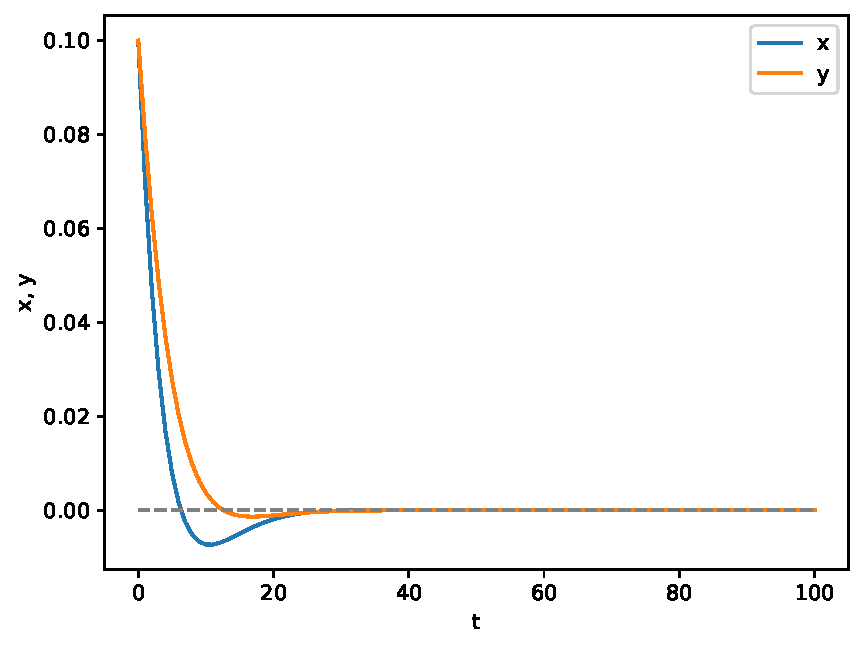
\includegraphics[scale=0.5]{figs/lin_sys.pdf}
		\caption{Dynamics of $x,y$ for the system \eqref{sys_lin_num}}
	\end{figure}
	
	
	 In studying the stability around the steady state, the eigenvalues of a Jacobian matrix provide valuable insights into the behavior of a dynamical system near its equilibrium points. They indicate how nearby trajectories behave over time. If the real parts of the eigenvalues are negative (i.e., the absolute value of the eigenvalues are less than 1), trajectories that start near the equilibrium point will converge towards it, indicating \textbf{stability}. If the real parts are positive, trajectories will diverge, leading to instability. 
	 
	\begin{ftheorem}
		Let the eigenvalues of the Jacobian matrix be $\lambda_1 \neq \lambda_2 \in \R$, then:
		\begin{enumerate}
			\item If $|\lambda_1| \leq |\lambda_2| < 1$, then
			\begin{align*}
				\text{ for all } 
				\begin{pmatrix}
						x_0 \\ y_0
				\end{pmatrix}, & \lim_{t\to\infty}  \begin{pmatrix}
				x_t \\ y_t
				\end{pmatrix} = 
				\begin{pmatrix}
				0 \\ 0
				\end{pmatrix}
			\end{align*}
			and the steady state $(0, 0)$ is \textbf{stable} in $\R^2$. Any value for $(x_0, y_0)$ will lead the
			dynamics to the steady state. The steady state $(0, 0)$ is said to be a \textbf{sink}. Furthermore. assume that $|\lambda_2| > |\lambda_1|$.
			\begin{itemize}
				\item if $\lambda_2 > 0$, the long run dynamics are monotonic
				\item if $\lambda_2 > 0$, the long run dynamics are oscillating.
			\end{itemize}
			\item If $|\lambda_2| \geq |\lambda_1| > 1$, all trajectories starting from
			\begin{align*}
				\begin{pmatrix}
					x_0 \\ y_0
				\end{pmatrix} \neq \begin{pmatrix}
				0 \\ 0
				\end{pmatrix}
			\end{align*}
			\textbf{explode}. The steady state $(0,0)$ is \textbf{unstable}. It is said to be a \textbf{source}.
			\item If $|\lambda_1| < 1 < |\lambda_2| $, there exists a unique direction along which the dynamics
			converge to $(0, 0)$. This implies that for a given $x_0$, there is only one value of $y_0$ such that the trajectory converges to the steady state. The steady state $(0, 0)$ is said to be a saddle point.
		\end{enumerate}
	\end{ftheorem}
	
	So far, we have assume that the 2 eigenvalues $\lambda_1, \lambda_2$ are real and not equal each other. The following analyzes such cases.
	
	\textbf{Repeated Eigenvalues}
	
	Write them as $\lambda_1 = \lambda_2 = \lambda$, then if
	\begin{enumerate}
		\item If $|\lambda < 1|$, all trajectories converge to $(0, 0)$, which is globally stable in $\R^2$.
		\item If $|\lambda > 1|$, all trajectories starting from $(x_0, y_0) \neq (0, 0)$ explode and $(0, 0)$ is unstable.
	\end{enumerate}
	
	\textbf{Complex Eigenvalues}
	
	We can write them as
	\begin{align*}
		\lambda_1 = \alpha + i \beta, \\
		\lambda_2 = \alpha - i \beta
	\end{align*}
	There are then two possibilities:
	\begin{enumerate}
		\item If $ \alpha^2 + \beta^2 = |\lambda_1|^2 = |\lambda_2|^2 < 1$, all trajectories converge to $(0, 0)$, which is globally stable in $\R^2$.
		\item If $ \alpha^2 + \beta^2 > 1$, all trajectories starting from $(x_0, y_0) \neq (0, 0)$ explode and $(0, 0)$ is unstable.
	\end{enumerate}
	
	\begin{example}
		Let's work through the stability analysis for the system \eqref{sys_lin_num}.
		
		\textbf{Step 1: Equilibrium Points}
		
		To find the equilibrium points, we need to solve the equations:
		\begin{align*}
			x_{t+1} &= x_t \\
			y_{t+1} &= y_t
		\end{align*}
		For the given system, the equilibrium points are found by setting each equation to its corresponding variable:
		\begin{align*}
			0.9x - 0.2y &= x \\
			0.1x + 0.7y &= y
		\end{align*}
		Solving these equations simultaneously, the equilibrium point is \((x^*, y^*) = (0, 0)\).
		
		\textbf{Step 2: Jacobian Matrix}
		
		The Jacobian matrix is given by:
		\[
		J =
		\begin{bmatrix}
			\dfrac{\partial f}{\partial x} & \dfrac{\partial f}{\partial y} \\
			\dfrac{\partial g}{\partial x} & \dfrac{\partial g}{\partial y}
		\end{bmatrix}
		\]
		Where $f$ and $g$ are the functions defining the system.
		
		For the given system, we have:
		\begin{align*}
			f(x, y) &= 0.9x - 0.2y \\
			g(x, y) &= 0.1x + 0.7y
		\end{align*}
		Calculating the partial derivatives, we get:
		\[
		J =
		\begin{bmatrix}
			0.9 & -0.2 \\
			0.1 & 0.7
		\end{bmatrix}
		\]
		
		\textbf{Step 3: Eigenvalues and Stability}
		
		Evaluate the Jacobian matrix at the equilibrium point \((0, 0)\):
		\[
		J^* =
		\begin{bmatrix}
			0.9 & -0.2 \\
			0.1 & 0.7
		\end{bmatrix}
		\]
		
		Calculate the eigenvalues of \(J^*\). The characteristic equation is given by:
		\[
		\det(J^* - \lambda I) = 0
		\]
		Solving this equation, we find that the eigenvalues are approximately \(0.8\) and \(0.8\).
		
		Since both eigenvalues have negative real parts, the equilibrium point \((0, 0)\) is stable.
		
		In conclusion, the equilibrium point \((0, 0)\) for the given system is stable due to the negative real parts of the eigenvalues of the Jacobian matrix.
		
	\end{example}	
	
	\subsection{System of 2 Nonlinear Difference Equations}
	We focus on the nonlinear dynamics, as they are the most common in economics.
	
	Consider the linear dynamics in $\R^2 \to \R^2$ following \eqref{sys_nonlin}. Given the initial state $(x_0, y_0)$. Assume that
	\begin{align}
		\begin{matrix}
			\bar{x} = f(\bar{x}, \bar{y}), \\
			\bar{y} = g(\bar{x}, \bar{y})
		\end{matrix} \label{sol_sys_nonlin}
	\end{align}
	be the steady state $(\bar{x}, \bar{y})$ of the system \eqref{sys_nonlin}. It is is locally stable if for any initial value $(x_0, y_0)$ near enough to $(\bar{x}, \bar{y})$, the dynamics starting from $(x_0, y_0)$ converge to $(\bar{x}, \bar{y})$. 
	
	Let us take a first-order Taylor expansion of $f(\cdot)$ around a steady state:
	\begin{align*}
		f(x,y) - f(\bar{x}, \bar{y}) \approx f'_x (\bar{x},\bar{y}) (x-\bar{x}) + f'_y (\bar{x},\bar{y}) (y-\bar{y})
	\end{align*}
	Similarly for $g(\cdot)$:
	\begin{align*}
		g(x,y) - g(\bar{x}, \bar{y}) \approx g'_x (\bar{x},\bar{y}) (x-\bar{x}) + g'_y (\bar{x},\bar{y}) (y-\bar{y})
	\end{align*}
	From \eqref{sys_nonlin},\eqref{sol_sys_nonlin}, we can write them in matrix form \footnote{This is called to ``linearize" around the steady state} as
	\begin{align}
		\begin{pmatrix}
			x_{t+1} - \bar{x} \\ y_{t+1} - \bar{y}
		\end{pmatrix}
		=  
		\underbrace{\begin{pmatrix}
			f'_x (\bar{x},\bar{y}) & f'_y (\bar{x},\bar{y}) \\ g'_x (\bar{x},\bar{y}) & g'_y (\bar{x},\bar{y})
		\end{pmatrix}}_{\J}
		\begin{pmatrix}
			x_{t} - \bar{x} \\ y_{t} - \bar{y}
		\end{pmatrix}
	\end{align}
	where, as well all know by now, $\J$ is the Jacobian matrix. The system has been ``linearized" and can be analyzed similarly to the linear case.
	
	\begin{ftheorem}
		Let $\lambda_1, \lambda_2$ be the eigenvalues of the Jacobian matrix $\J$ evaluated at the steady state $(\bar{x}, \bar{y})$. Then
		\begin{enumerate}
			\item If $|\lambda_1| \leq |\lambda_2| < 1$, the steady state is locally stable. Any initial condition will lead the dynamics to the steady state. The steady state $(\bar{x}, \bar{y})$ is said to be a \textbf{sink}.
			\item If $|\lambda_1| \geq |\lambda_2| > 1$, the steady state is unstable: for any initial condition different from the steady state, the trajectories are locally exploding. The steady state is said to be a \textbf{source}.
			\item If $|\lambda_1| < 1 < |\lambda_2| $, the steady state is a saddle point. For a given initial con- dition on one variable, there is only one initial value of the other variable such that the trajectory converges to the steady state. Any other value for this variable would lead the trajectory to locally explode.
		\end{enumerate}
		When the eigenvalues are real and their moduli (absolute value) lie on the same side of 1, the steady state is also called a (stable or unstable) \textit{node}.
	\end{ftheorem}
	
	From a practical point of view, it is often easier to use the \textbf{trace} ($\T$) and the \textbf{determinant}($\D$) of the Jacobian matrix. The results are summarized as follows.
	\begin{ftheorem}
		We have
		\begin{align*}
			\T = tr(\J) = f'_x + g'_y 
		\end{align*}
		and
		\begin{align*}
			  \D  = \det(\J)  =  f'_x g'_y - f'_y g'_x 
		\end{align*}
		Then:
		\begin{enumerate}
			\item If $| 1 + \D | < |\T|$, the steady state is a saddle. 
			\item If $|1+\D| > |\T|$ and $|\D| < 1$, the steady state is a sink.
			\item If $|1+\D| > |\T|$ and $\D| > 1$, the steady state is a source.
		\end{enumerate}
	\end{ftheorem} 
	
	\section{Problem Sets}
	The following exercises are from \citet[p.395--399]{sydsaeter2008further}.
	\begin{ex}
		Find the solution and equilibrium point
		\begin{align*}
			(a)\ & x_{t+1} = 2 x_t + 4, \ x_0 = 1, \\
			(b)\ & 3 x_{t+1} = x_t +2, \ x_0 = 2, \\
			(c)\ & 2 x_{t+1} + 3 x_t + 2 = 0, \ x_0 = -1, \\
			(d)\ & x_{t+1} - x_t + 3 = 0, \ x_0 = 3
		\end{align*}
	\end{ex}
	
	\begin{ex}[Cobweb Model]
		Assume the total cost of raising $q$ pigs is
		\begin{align*}
			C(q) = \alpha q + \beta q^2
		\end{align*}
		Suppose there are $N$ identical pig farms. Let the demand function for pigs be
		\begin{align*}
			D(p) = \gamma - \delta p
		\end{align*}
		where $p$ is the price, $\alpha,\beta,\gamma,\delta$ are positive constants. Each farmer behaves competitively and taking price as given to maximize their profit according to
		\begin{align*}
			\pi(q) = pq - C(q)
		\end{align*}
		\begin{enumerate}
			\item Find the quantity $q^*$ that maximizes profit.
			\item Find the Aggregate Supply $S(p)$.
			\item Now, suppose it takes 1 period to raise each pig. When choosing the number of pigs to raise for sale at time $t+1$, each farmer remembers the price $p_t$ and expect $p_{t+1}$ to be the same as $p_t$. Thus, aggregate supply at time $t+1$ is $S(p_t)$. Find the equilibrium price satisfying
			\begin{align*}
				S(p_t) = D(p_{t+1})
			\end{align*}
			\item Write solution of $p_t$ in terms of $p_0$ and a time path.
			\item Find the equilibrium. Analyze its stability. When is it stable? When is it not?
		\end{enumerate}
	\end{ex}	
		
	\chapter{Static Optimization and Economic Modeling}
	\section{Unconstraint Optimization}
	Say we want to find the solutions of $n$ choice variables ($\x = (x_1, \dots, x_n)$ )
	\begin{align*}
		\max_{\x} F(\x) 
	\end{align*}
	
	\begin{figure}[ht]
		\centering
		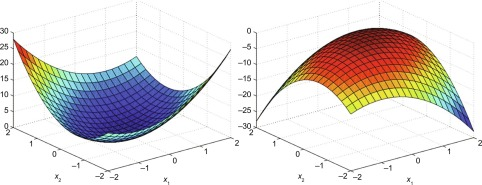
\includegraphics[scale=1]{figs/maxmin.jpg}
		\caption{Find the min (left) or max (right).}
	\end{figure}
	
	\subsection{Necessary Conditions}
	This condition requires that the solution $\x^*$ must be a critical point of $f$, that is $f'(\x^*)=0$. $\x^*$ will not be the endpoint of the interval under consideration, which means it lies in the INTERIOR of the domain of $f$. 
	
	\begin{ftheorem}
		Let $F: U \mapsto \R^1$ be a $C^1$ function defined on a subset $U$ of $\R^n$. If $\x^*$ is a local max or min of $F$ in $U$, and if $\x^*$ is an interior point of $U$, then
		\begin{equation*}
			\frac{\partial F}{\partial x_i} (\x^*) = 0 \ \text{for $i = 1, \dots, n$ }
		\end{equation*}
	\end{ftheorem}
	Basically, the FOCs to every choice variable must be 0. We can write the condition in the form of Jacobian
	\begin{equation*}
		D F(\x^*) = 
		\begin{pmatrix}
			\dfrac{\partial F}{\partial x_1} (\x^*)            & \dots  & \dfrac{\partial F}{ \partial x_n} (\x^*) 
		\end{pmatrix} = \0
	\end{equation*}
	The solution $\x^* \neq 0$ for this problem is called a ``non-trivial solution". Otherwise, if $\x^* = 0$, then it is called a ``trivial" or corner solution, which is usually uninteresting in economics.
	
	\subsection{Sufficient Conditions}
	We need to use a condition on the second derivatives of $F$ to determine whether the critical point is a max or a min. A $C^2$ function of $n$ variables has $n^2$ second-order partial derivatives at each point in its domain. We combine them into a $n\times n$ matrix called the \textbf{Hessian} of $F$
	\begin{equation*}
		D^2 F(\x^*) = 
		\begin{pmatrix}
			\dfrac{\partial^2 F}{\partial x_1^2} (\x^*)            & \dots  & \dfrac{\partial^2 F}{\partial x_1 \partial x_n} (\x^*) \\
			\vdots                                                 & \ddots & \vdots                                                 \\
			\dfrac{\partial^2 F}{\partial x_n \partial x_1} (\x^*) & \dots  & \dfrac{\partial^2 F}{\partial x_n^2} (\x^*)            
		\end{pmatrix}
	\end{equation*}
	The Hessian is always a symmetric matrix. Whether the critical point is a min or max or neither depends on the definiteness of the Hessian matrix at that point.
	
	\begin{ftheorem}
		Let $F: U \mapsto \R^1$ be a $C^2$ function whose domain is an open set $U$ in $\R^n$. Suppose that $\x^*$ is a critical point of $F$, then
		\begin{enumerate}
			\item If the Hessian $D^2 F(\x^*)$ is a NEGATIVE DEFINITE symmetric matrix, then $\x^*$ is a strict LOCAL MAX of $F$,
			\item If the Hessian $D^2 F(\x^*)$ is a POSITIVE DEFINITE symmetric matrix, then $\x^*$ is a strict LOCAL MIN of $F$,
			\item If the Hessian $D^2 F(\x^*)$ is INDEFINITE, then $\x^*$ is neither a local max nor a local min of $F$.
		\end{enumerate}
	\end{ftheorem}
	
	In general, there are 2 methods to test for definiteness.
	
	\subsubsection{(1) The Signs of the Leading Minors}
	\begin{ftheorem}[Sufficient Conditions for a MAX]
		Let $F: U \mapsto \R^1$ be a $C^2$ function whose domain is an open set $U$ in $\R^1$. Suppose that
		\begin{equation*}
			\frac{\partial F}{\partial x_i} (\x^*) = 0 \ \text{for $i = 1, \dots, n$ }
		\end{equation*}
		and that the $n$ leading principal minors of $D^2 F(\x^*)$ \underline{alternate in sign}
		\begin{align*}
			|F''_{x_1 \ x_1}| < 0, 
			\begin{vmatrix}
				F''_{x_1 \ x_1} & F''_{x_2 \ x_1} \\
				F''_{x_1 \ x_2} & F''_{x_2 \ x_2} 
			\end{vmatrix} > 0,
			\begin{vmatrix}
				F_{x_1 \ x_1} & F_{x_2 \ x_1} & F_{x_3 \ x_1} \\
				F_{x_1 \ x_2} & F_{x_2 \ x_2} & F_{x_3 \ x_2} \\
				F_{x_1 \ x_3} & F_{x_2 \ x_3} & F_{x_3 \ x_3} 
			\end{vmatrix} < 0, \dots
		\end{align*}
		at $\x^*$. Then $\x^*$ is a strict local max of $F$.
	\end{ftheorem}
	
	\begin{ftheorem}[Sufficient Conditions for a MIN]
		Let $F: U \mapsto \R^1$ be a $C^2$ function whose domain is an open set $U$ in $\R^1$. Suppose that
		\begin{equation*}
			\frac{\partial F}{\partial x_i} (\x^*) = 0 \ \text{for $i = 1, \dots, n$ }
		\end{equation*}
		and that the $n$ leading principal minors of $D^2 F(\x^*)$ \underline{all positive}
		\begin{align*}
			|F_{x_1 \ x_1}| > 0, 
			\begin{vmatrix}
				F_{x_1 \ x_1} & F_{x_2 \ x_1} \\
				F_{x_1 \ x_2} & F_{x_2 \ x_2} 
			\end{vmatrix} > 0,
			\begin{vmatrix}
				F_{x_1 \ x_1} & F_{x_2 \ x_1} & F_{x_3 \ x_1} \\
				F_{x_1 \ x_2} & F_{x_2 \ x_2} & F_{x_3 \ x_2} \\
				F_{x_1 \ x_3} & F_{x_2 \ x_3} & F_{x_3 \ x_3} 
			\end{vmatrix} > 0, \dots
		\end{align*}
		at $\x^*$. Then $\x^*$ is a strict local min of $F$.
	\end{ftheorem}
	
	\begin{figure}[ht]
		\centering
		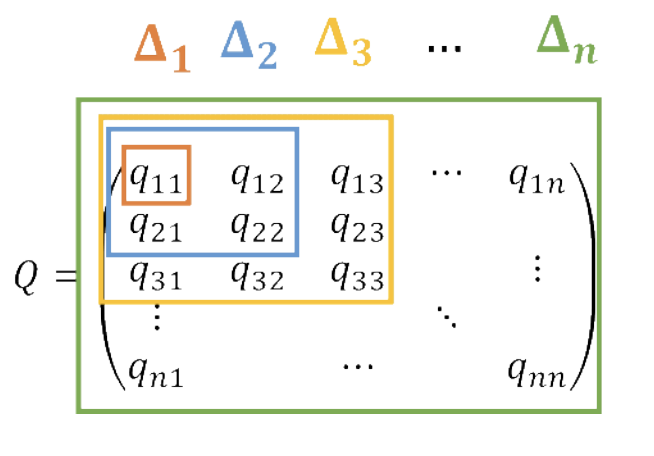
\includegraphics[scale=0.4]{prinminors.png}
		\caption{Principal Minors}
	\end{figure}
	
	\subsubsection{(2) The Signs of the Eigenvalues}
	Another way is to evaluate the Eigenvalues of the Hessian at critical points. 
	
	\begin{ftheorem}[Eigenvalues Test for Sufficient Conditions]
		If the Hessian at a given point has \textbf{all positive eigenvalues}, it is said to be positive-definite, meaning the function is \textbf{concave up (convex)} at that point. If all the \textbf{eigenvalues are negative}, it is said to be a negative-definite, equivalent to \textbf{concave down}.
	\end{ftheorem}
	
	To find the eigenvalues $\lambda$ of a matrix $\A$, solve the following
	\begin{align*}
		 \det (\A - \lambda \I) = 0      
	\end{align*}
	
	\begin{figure}[ht]
		\centering
		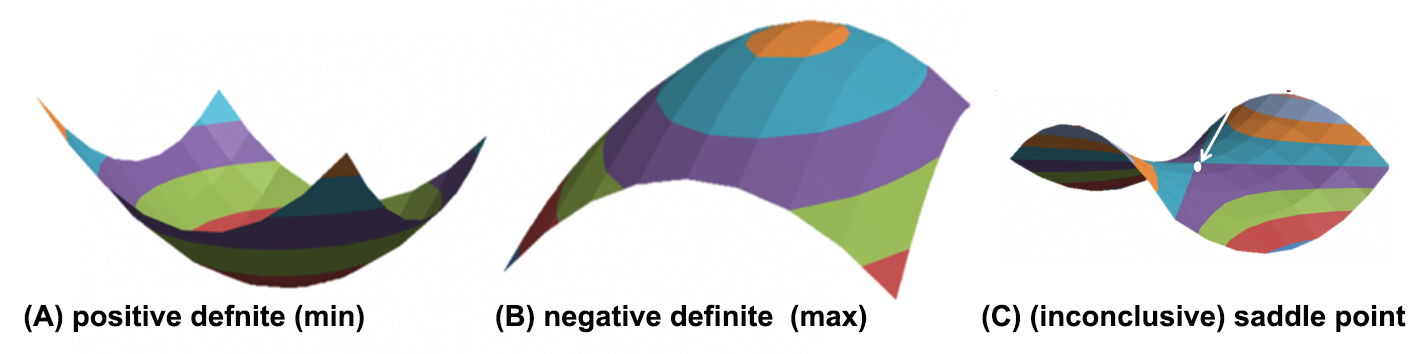
\includegraphics{figs/hessian.png}
		\caption{The definiteness of the Hessian matrix}
	\end{figure}
	
	Intuitively, a negative definite Hessian matrix at the optimal point suggests that the objective function is concave in the vicinity of that point. This means that the function curves downward and resembles a bowl-like shape around the optimal point. In other words, if you move a little bit away from the optimal point in any direction, the function value will decrease. This curvature indicates that you are on the highest point in that particular region, and there is no other point nearby that can provide a higher value for the function. Mathematically, a matrix is negative definite if all its eigenvalues are negative. In the context of the Hessian matrix, the negative eigenvalues indicate that the curvature of the function in the corresponding directions is downward, which aligns with the idea of concavity.
	
	\subsection{Examples}
	
	\begin{example}[Optimization]
	\label{ex:soc2}
		Suppose
		\begin{align*}
			f(x,y) = x^4 + y^2 - xy 
		\end{align*}
		The critical point is found by
		\begin{align*}
			& (x): \frac{\partial f}{\partial x} = 4x^3 - y = 0 \iff y  = 4 x^3, \\
			& (y): \frac{\partial f}{\partial y} = 2y - x = 0 \iff y = x/2.      
		\end{align*}
		Solving for $x$ yields the following critical points
		\begin{align*}
			(x^*,y^*) = (0,0), \ (\frac{1}{2\sqrt{2}} , \frac{1}{4\sqrt{2}}  ), \ (-\frac{1}{2\sqrt{2}} , -\frac{1}{4\sqrt{2}}  ) 
		\end{align*}
		To verify the extremum, we evaluate the Hessian matrix at the critical points
		\begin{align*}
			H = \begin{pmatrix}
				12 x^2 & -1 \\
				-1     & 2  
			\end{pmatrix}
		\end{align*}
		The first principal minor is $12x^2$. The second principal minor is $H$ itself where
		\begin{align*}
			| H | = 24 x^2 - 1 
		\end{align*} 
		Thus, we conclude that $(0,0)$ is a saddle point. 
		
		The other 2 critical points $(\frac{1}{2\sqrt{2}} , \frac{1}{4\sqrt{2}}  ), \ (-\frac{1}{2\sqrt{2}} , -\frac{1}{4\sqrt{2}}  )$ are minima.
	\end{example}
	
	\begin{example}
		Consider the maximization problem
		\begin{align*}
			\max \ f(x) = - x^2 + 2ax + 4 a^2 
		\end{align*}
		What is the effect of an increase in $a$ on the maximal value of $f(x,a)$?
		
		First, Find the critical point. Taking FOC yields $x^* = a$
		\begin{enumerate}
			\item (Direct Solution) Inserting to the objective function $f(a) = 5 a^2$ and so the effect of $a$ on $f$ is $df/da = 10a$. \\
			\item (Envelop Theorem) 
			\begin{align*}
				f'(a) = \frac{\partial f}{\partial a} = 2x + 8a 
			\end{align*}
			evaluate at $x=a$ also yields $10a$.
		\end{enumerate}
	\end{example}
	
	\subsection{Problem Sets}
	
	\begin{ex}
		Find the optimal solution for
		\begin{align*}
			(a) & \ \min_x x^2 - 4x + 7, \\
			(b) & \ \max_x \ln(x+1) \text{ for $x \geq 0$} \\
			(c) & \ \max_x x^3 - 6x^2 + 9x \text{ for $x \in [-1,4]$} \\
			(d) & \ \max_x [800x - 2x^2] - (100 + 150 x)
		\end{align*}
	\end{ex}
	
	\begin{ex}
		Find the eigenvalues and evaluate them at given points, and determine whether the matrix is negative-definite, positive-definite, or indefinite.
		\begin{align*}
			(a) &\begin{pmatrix}
				12 x^2 & -1   \\ -1 & 2
			\end{pmatrix} \ \ \text{at} \ (3,1), \\
			(b) &\begin{pmatrix}
				6x     & 0    \\ 0 & 6y
			\end{pmatrix} \ \ \text{at} \ (-1,2), \\
			(c) &\begin{pmatrix}
				-2y^2  & -4xy \\ -4xy & -2 x^2
			\end{pmatrix} \ \ \text{at} \ (1,-1) \ \ \text{and} \ \ (1,0) \\
		\end{align*}
	\end{ex}
	

	
	\begin{ex}
		Find the optimal solutions for
		\begin{align*}
			(a) &\ \max_{x,y} f(x,y) = -2 x^2 - 3 y^2 + 4xy \\
			(b) &\ \max_{x,y} f(x,y) = -x^3 - 2y^3 + 3xy \\
			(c) &\ \min_{x,y,z} f(x,y,z) = x^2 + 6xy + y^2 - 3yz + 4z^2 - 10x - 5y - 21z.
		\end{align*}
		Verify with SOC condition.
	\end{ex}


	\begin{ex}
	Endogenous Fertility \citep{de2012fertility} p.12.
		\begin{align*}
			 \max_{s_t, n_t}  \ln (w(1-\phi n_t) - s_t) + \beta \ln((1+r)s_t) + \gamma \ln (n_t)
		\end{align*}
		where $n$ is fertility decision, $\phi$ is the time-cost of raising children, $s, w, r$ are savings, wage rate, and interest rate.
		\begin{enumerate}
			\item Find the optimal fertility decision.
			\item Add a good cost of childcare per child (say $\theta > 0$), will it change the fertility decision?
		\end{enumerate}
	\end{ex}
	
	\begin{ex} Endogenous Fertility with Bequest \citep{de2012fertility} p.189.
		\begin{align*}
			\max_{l_t,n_t,b_t}  \ln ( (1-l_t-\phi N_t^\sigma n_t)k_t - n_t b_t) + \varphi \ln (l_t) + \gamma  \ln(n_t k_{t+1} )
		\end{align*}
		where $l_t, n_t, b_t$ are leisure, fertility, and educational bequests. The idea is that population size asserts a negative externality on having children.
		
		Productive assets accumulate according to
		\begin{align*}
			k_{t+1} = \mu b_t^\eta k_t^\tau
		\end{align*}
		
		\begin{enumerate}
			\item Write the first-order conditions.
			\item Find the optimal values $l^*, n^*, b^*$.
		\end{enumerate}
	\end{ex}
	
	\begin{ex}
		Principal-Agent problem \citep{varian1992microeconomic}, p.453
		
		The Agent's problem is
		\begin{align*}
			\max_a \delta + \gamma a - \frac{\gamma^2 r}{2} \sigma^2 - c(a)
		\end{align*}
		where $a$ is the agent's effort.
		The Principal's problem is
		\begin{align*}
			\max_{\delta,\gamma, a} (1-\gamma)a - \delta 
		\end{align*}
		where $\delta + \gamma a - \dfrac{\gamma^2 r}{2} \sigma^2 - c(a) = 0$. Let $c(a)$ be a convex function.
		\begin{enumerate}
			\item Solve the Agent's problem to obtain $a$
			\item For the Principal's problem, first, extract $\delta$ as a function of $\gamma,a$. Then, replace it back to the objective function, use the results from 1. and solve for $a$.
			\item Assume $c(a) = 0.5 a^2$. Derive the explicit solution.
		\end{enumerate}
	\end{ex}
	
	\newpage	
	\section{Constraint Optimization}
		Let us consider an optimization problem for $n$ variables with $k$ constraints s.t.
	\begin{align*}
		& \max_{\x} (\min) f \underbrace{(x_1, \dots, x_n)}_{\x} \\
		s.t. &\ h_i (\x) = c_i \ \text{ for } \ i = 1, \dots, k. &                                                        
	\end{align*}
	
	\begin{figure}[ht]
		\centering
		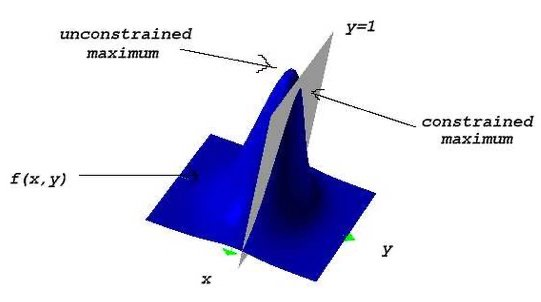
\includegraphics[scale=0.7]{figs/cons_vs_uncons.jpg}
		\caption{An example of Constraint Optimization}
	\end{figure}
		
	\subsection{Necessary First-order Conditions}
	Assume that NDQC is satisfied. There will be $k$ Lagrangian multipliers $\lambda_i$ for  $i = 1, \dots, k$. The Lagrangian is
	\begin{align*}
		\mathcal{L} (\x, \lambda_i) = f(\x) - \sum^k_{i=1} \lambda_i (h_i(\x) - c_i) 
	\end{align*}
	As usual, the FOC is just
	\begin{align*}
		\frac{\partial \mathcal{L}}{\partial x_i} = 0  \ \ \text{ for $i=1,\dots,n$}
	\end{align*}
	
	Let us show what it means in a problem of 1 function of 2 variables.
		\begin{ftheorem}
		Let $f$ and $h$ be $C^1$ functions of 2 variables. Suppose that $\x^* = (x^*_1, x^*_2)$ is a solution of the problem
		\begin{align*}
			& \max f(x_1,x_2)   \\
			s.t. & \ h(x_1, x_2) = c 
		\end{align*}
		Suppose further that $(x^*_1, x^*_2)$ is not a critical point of $h$. Then, there is a real number $\lambda^*$ such that $(x^*_1, x^*_2, \lambda^*)$ is a critical point of the Lagrangian function
		\begin{align*}
			\mathcal{L} (x_1, x_2, \lambda) \equiv f(x_1, x_2) - \lambda [ h(x_1, x_2) - c]. 
		\end{align*}
		In other words, at $(x^*_1, x^*_2, \lambda^*)$ we can obtain the First-order conditions 
		\begin{align*}
			\frac{\partial \mathcal{L}}{\partial x_1} = 
			\frac{\partial \mathcal{L}}{\partial x_2} = 
			\frac{\partial \mathcal{L}}{\partial \lambda} = 0.
		\end{align*}
		or
		\begin{align*}
			\nabla \mathcal{L} (x_1, x_2, \lambda) = 0
		\end{align*}
	\end{ftheorem}
	
		\begin{example}
		The problem is
		\begin{align*}
			& \max_{x,y} \ f(x,y) = xy \\
			s.t. & \ 2x + y = 100           
		\end{align*}
		
		\textbf{Method 1: Lagrangian Method}
		
		
		The Lagrangian is
		\begin{align*}
			\mathcal{L} = xy - \lambda (2x + y - 100) 
		\end{align*}
		The FOCs:
		\begin{align*}
			& \mathcal{L}'_x = y - 2\lambda = 0,       \\
			& \mathcal{L}'_y = x - \lambda = 0,        \\
			& \mathcal{L}'_\lambda = 2x + y - 100 = 0, 
		\end{align*}
		which yields the solution $(x^*,y^*) = (25,50)$. 
		
		\textbf{Method 2: Substitution Method or ``Naive" Method}
		
		
		We can turn the constrained optimization problem into an unconstrained problem. From the constraint, we have $y = 100 -x$, the problem becomes
		\begin{align*}
			\max_{x} x (100-2x) 
		\end{align*}
		The FOC is
		\begin{align*}
			100 - 4x = 0, 
		\end{align*}
		which also gives $x^*=25, y^* = 50$.
		
	\end{example}

	
	\subsection{Sufficient Conditions}
	For sufficient conditions, we need to use the notion of Bordered Hessian Matrix. The construction of such a matrix is
	\begin{equation*}
		H = \left( \begin{array}{c | c}
			\begin{matrix}
				0      & \dots  & 0      \\
				\vdots & \ddots & \vdots \\
				0      & \dots  & 0      
			\end{matrix} & 
			\begin{matrix}
				B_{11} & \dots  & B_{1n} \\
				\vdots & \ddots & \vdots \\
				B_{m1} & \dots  & B_{mn} 
			\end{matrix} \\
			\hline
			\begin{matrix}
				B_{11} & \dots  & B_{m1} \\
				\vdots & \ddots & \vdots \\
				B_{1n} & \dots  & B_{mn} 
			\end{matrix} & 
			\begin{matrix}
				a_{11} & \dots  & a_{1n} \\
				\vdots & \ddots & \vdots \\
				a_{1n} & \dots  & a_{nn} 
			\end{matrix}
		\end{array} \right)
	\end{equation*}
	in short, it looks like this
	\begin{align*}
		H = \begin{pmatrix}
			0 & \B \\ \B^T & \L
		\end{pmatrix}
	\end{align*}
	where $\B$ is the matrix of derivatives of constraints $h_i$ wrt to $\x$, and $\L$ is the matrix of second-order derivatives of the Lagrangian $\mathcal{L}$ wrt to $\x$. 
	
	In our case, it looks like this
	\begin{equation*}
		H = \left( \begin{array}{c | c}
			\begin{matrix}
				0      & \dots  & 0      \\
				\vdots & \ddots & \vdots \\
				0      & \dots  & 0      
			\end{matrix} & 
			\begin{matrix}
				\frac{\partial h_1}{\partial x_1} & \dots  & \frac{\partial h_1}{\partial x_n} \\
				\vdots                            & \ddots & \vdots                            \\
				\frac{\partial h_k}{\partial x_1} & \dots  & \frac{\partial h_k}{\partial x_n} 
			\end{matrix} \\
			\hline
			\begin{matrix}
				\frac{\partial h_1}{\partial x_1} & \dots & \frac{\partial h_k}{\partial x_1} \\
				\vdots                            & \ddots & \vdots                            \\
				\frac{\partial h_1}{\partial x_n} & \dots  & \frac{\partial h_k}{\partial x_1} 
			\end{matrix} & 
			\begin{matrix}
				\frac{\partial^2 \mathcal{L}}{\partial x_1^2}            & \dots  & \frac{\partial^2 \mathcal{L}}{\partial x_1 \partial x_n} \\
				\vdots                                                   & \ddots & \vdots                                                 \\
				\frac{\partial^2 \mathcal{L}}{\partial x_n \partial x_1} & \dots  & \frac{\partial^2 \mathcal{L}}{\partial x_n^2}          
			\end{matrix}
		\end{array} \right)
	\end{equation*}
	This $(k+n) \times (k+n)$ matrix has $k+n$ leading principal minors (the biggest one is $H$ itself). The first $m$ matrices $H_1, \dots , H_k$ are zero matrices. The next  $k - 1$ matrices $H_{k+1}, \dots , H_{2k-1}$ have zero determinant.
	
	The determinant of the next minor $H_{2k}$ is $\pm \det(H')^2$ where $H'$ is the upper $k \times k $ minor of $H$ after block of zeros, so $\det H_{2k}$ does not contain information about $f$.
	
	And only the determinants of the last $n - k$ leading principal minors 
	\begin{align*}
		H_{2k+1}, H_{2k+2}, \dots , H_{2k+(n - k) = k + n} \equiv H 
	\end{align*}
	carry information about both, the objective function $f$ and the constraints $h_i$. Exactly these minors are essential for the following sufficient condition for constraint optimization.
	
	
	
	\begin{ftheorem}[Constraint SOC]
		Suppose $\x^*$ satisfies the FOCs.
		\begin{enumerate}
			\item For the bordered Hessian matrix $H$, the last $n-k$ leading principal minors 
			\begin{align*}
				H_{2k+1}, H_{2k+2}, \dots , H_{2k+(n - k) = k + n} \equiv H 
			\end{align*}
			evaluated at the critical point ALTERNATE in signs where the last minor $H_{n+k} \equiv H$ has the sign as $(-1)^n$, then $\x^*$ is a LOCAL MAX.
			\item For the bordered Hessian matrix $H$, the last $n-k$ leading principal minors 
			\begin{align*}
				H_{2k+1}, H_{2k+2}, \dots , H_{2k+(n - k) = k + n} \equiv H 
			\end{align*}
			evaluated at the critical point have the SAME sign where the last minor $H_{n+k} \equiv H$ has the sign as $(-1)^k$, then $\x^*$ is a LOCAL MIN.
		\end{enumerate} \label{theorem:soc_constraint}
	\end{ftheorem}
	which can be summarized as
	\begin{table}[ht]
		\centering
		\begin{tabular}{c | c | c | c | c | c}
			\hline
			& $H_{2k+1}$   & $H_{2k+2}$   & $\dots$ & $H_{k+n-1}$  & $H_{k+n} \equiv H$ \\
			\hline
			$\max$ & $(-1)^{k+1}$ & $(-1)^{k+2}$ & $\dots$ & $(-1)^{n-1}$ & $(-1)^n$           \\
			$\min$ & $(-1)^k$     & $(-1)^k$     & $\dots$ & $(-1)^k$     & $(-1)^k$           \\
			\hline
		\end{tabular}
	\end{table}
	
	We provide here only the sufficient conditions for a problem of \textbf{2 variables and 1 constraint}, which is the most common.
	
	\begin{ftheorem}
		Let $f,h$ be $C^2$ functions on $\R^2$. Consider the problem
		\begin{align*}
			\max_{x,y} f(x,y) \ \textbf{ s.t. } h(x,y) = c  \ \text{ for } c \in C_h \text{(constraint set)} 
		\end{align*}
		The Lagrangian is
		\begin{align*}
			\mathcal{L}(x,y,\lambda) = f(x,y) - \lambda (h(x,y) - c) 
		\end{align*}
		Suppose that $(x^*, y^*, \lambda^*)$ satisfies the following FOCs
		\begin{align*}
			\mathcal{L}'_x = \mathcal{L}'_y = \mathcal{L}'_\lambda = 0 \ \ \text{ at $(x^*,y^*,\lambda^*)$} 
		\end{align*}
		and the bordered Hessian matrix is
		\begin{align*}
			H = \begin{pmatrix}
				0                             & \frac{\partial h}{\partial x}                        & \frac{\partial h}{\partial y}                        \\
				\frac{\partial h}{\partial x} & \frac{\partial^2 \mathcal{L}}{\partial x^2}          & \frac{\partial^2 \mathcal{L}}{\partial x \partial y} \\
				\frac{\partial h}{\partial y} & \frac{\partial^2 \mathcal{L}}{\partial y \partial x} & \frac{\partial^2 \mathcal{L}}{\partial y^2}          
			\end{pmatrix}
		\end{align*}
		\begin{enumerate}
			\item 		if $\det(H) > 0$ at $(x^*, y^*)$, then $(x^*, y^*)$ is the local MAX of $f$ on $C_h$.
			\item 		if $\det(H) < 0$ at $(x^*, y^*)$, then $(x^*, y^*)$ is the local MIN of $f$ on $C_h$.
		\end{enumerate}
	\end{ftheorem}
	
	\subsection{Examples}
	
		\begin{example}[1 objective function of 2 variables and 1 constraint]
		
		Find the extremum of
		\begin{align*}
			& F(x,y) = xy          \\
			s.t. &\ h(x,y) = x+ y = 6. &                      
		\end{align*}
		The Lagrangian is
		\begin{align*}
			L(x,y) = xy - \lambda (x+y-6) 
		\end{align*}
		The FOCs are
		\begin{align*}
			& (x): \frac{\partial L}{\partial x} = y - \lambda = 0,           \\
			& (y): \frac{\partial L}{\partial y} = x - \lambda = 0,           \\
			& (\lambda): \frac{\partial L}{\partial \lambda} = x + y - 6 = 0, 
		\end{align*}
		which gives
		\begin{align*}
			x^* = y^* = 3, \ \lambda = 3 
		\end{align*}
		To tell the nature of its extremum, we test the second-order conditions. The bordered Hessian is
		\begin{align*}
			H = \begin{pmatrix}
				0 & 1 & 1 \\
				1 & 0 & 1 \\
				1 & 1 & 0 
			\end{pmatrix}
		\end{align*}
		We have $n=2, k=1$ so we have to check the $n-k=1$ last leading principal minors, a.k.a, $H$ itself. Calculation shows that $\det H = 2 > 0$ has the same sign with $(-1)^n = (-1)^2 > 0$ so our critical point is a MAX. 
	\end{example}
	
		\begin{example}[1 objective function of 2 variables and 2 constraint]
		Find the extremum of
		\begin{align*}
			& F(x,y,z) = x^2 + y^2 + z^2     \\
			s.t. &\ h_1(x,y,z) = 3x + y + z = 5, &                                \\
			& \  h_2 (x,y,z) = x + y + z = 1 
		\end{align*}
		The Lagrangian is
		\begin{align*}
			L(x,y) = x^2 + y^2 + z^2 - \lambda_1 (3x + y + z - 5) - \lambda_2 (x + y +z - 1) 
		\end{align*}
		The FOCs are
		\begin{align*}
			& (x): \frac{\partial L}{\partial x} = 2x - 3 \lambda_1 - \lambda_2  = 0,  \\
			& (y): \frac{\partial L}{\partial y} = 2y - \lambda_1 - \lambda_2 = 0,     \\
			& (z): \frac{\partial L}{\partial z} = 2z - \lambda_1 - \lambda_2 = 0,     \\
			& (\lambda_1): \frac{\partial L}{\partial \lambda_1} = 3x + y + z - 5 = 0, \\
			& (\lambda_2): \frac{\partial L}{\partial \lambda_2} = x + y +z - 1 = 0    
		\end{align*}
		which gives
		\begin{align*}
			x^* = 2, \ \ y^* = - 1/2, \ \ z^* = -1/2, \ \ \lambda_1 = 5/2, \ \ \lambda_2 = -7/2 
		\end{align*}
		To tell the nature of its extremum, we test the second-order conditions. The bordered Hessian is
		\begin{align*}
			H = \left( \begin{array}{c | c}
				\begin{matrix}
					0 & 0 \\
					0 & 0 
				\end{matrix} & \begin{matrix}
					3 & 1 & 1 \\
					1 & 1 & 1 
				\end{matrix} \\
				\hline
				\begin{matrix}
					3 & 1  \\
					1 & 1  \\
					1 & 1 
				\end{matrix} & \begin{matrix}
					2 & 0 & 0 \\
					0 & 2 & 0 \\
					0 & 0 & 2 
				\end{matrix}
			\end{array} \right)
		\end{align*}
		We have $n=3, k=2$ so we have to check the $n-k=1$ last leading principal minors, a.k.a, $H$ itself. Calculation shows that $\det H = 16 > 0$ has the same sign with $(-1)^k = (-1)^2 > 0$ so our critical point is a MIN. 
	\end{example}
	
	\subsection{Problem Sets}
	
	\begin{ex}
		Find the extremum, then verify it is either max or min.
		\begin{align*}
			& (a) \ f(x,y) = 7 - y - x^2  && \text{ s.t} && h(x,y) = x + y =0; \\
			& (b) \ f(x,y) = x(y+4) && \text{ s.t} && h(x,y) = x + y = 8; \\
			& (c) \ x_1^2+x_2^2+x_3^2 && \text{ s.t} && x_1+x_2+x_3=1; \\
			& (d) \ yz + xz && \text{ s.t} && y^2 + z^2 = 1, \ xz=3.
		\end{align*}
	\end{ex}
	
	\begin{ex}[Beckerian trade-off] \label{ex:ferti}
		A parent's problem is
		\begin{align*}
			\max_{c_t, d_{t+1}, n_t, e_t} & \ln(c_t) + \beta \ln (d_{t+1}) + \gamma \ln ( \Pi_t n_t) \\
			\text{s.t.}\ & c_t + s_t +e_tn_t = (1-\phi n_t) w_t, \\
			& d_{t+1} = (1+r_{t+1}) s_t, \\
			& \Pi_t = (\theta + e_t)^\eta
		\end{align*}
		where $c,d,s,n,e$ are consumption when young, consumption when old, saving, number of children, and children's education. The parameters $\beta,\gamma,\phi,\theta,\eta \in (0,1)$. This problem is a simplified version of the model in \citet{de2012fertility}, p.22. 
		\begin{enumerate}
			\item Find the optimal solutions.
			\item (if time allows) verify by constructing a Hessian (you should use the Naive method)
			\item Is there a trade-off between children's quantity and quality?
		\end{enumerate}
	\end{ex}
	
	\begin{ex}[Renewable Resources] \label{ex:rr}
		Section 9.2 of \citet{farmer2010intertemporal} (p.120). A country has a stock of renewable resource $R_t$ such that
		\begin{align*}
			R_{t+1} = R_t + g(R_t) - X_t
		\end{align*}
		where $g(R_t)$ is the rate of regeneration, while $X_t$ is harvested stock (think of fish). We can assume a simple regenerate form
		\begin{align*}
			g(R_t) = \delta R_t - \gamma R_t^2 \text{ where $\delta > 1, \gamma < 1$}
		\end{align*}
		Household's budget constraint when young is
		\begin{align*}
			c_t + k_{t+1} + p_t R_t = q_t X_t + w_t
		\end{align*}
		LHS: expenses, including hoarding renewable resources. LHS: harvest then sell + wage. When old, his constraint is
		\begin{align*}
			d_{t+1} = (1+r) k_{t+1} + p_{t+1} R_{t+1}
		\end{align*}
		Utility function is $\ln(c_t) + \beta \ln(d_{t+1})$. Household's choice variables are $c_t, d_{t+1}, X_t, R_t$. Find the optimal solutions by forming the Lagrangian and take the FOC wrt all the choice variables.
	\end{ex}

		\begin{ex}[New Technology] 
		Without technology, a country solves
		\begin{align*}
			\max &\log(c_0) + \beta \log(c_1), \\
			s.t. & c_0 + k_1 = f(k_0), \\
			&c_1 = f(k_1)
		\end{align*}	
		If she invests in new technology, she solves
		\begin{align*}
			\max &\log(c_0) + \beta \log(c_1), \\
			s.t. & c_0 + s_0 = f(k_0), \\
			& s_0 = k_1 + \lambda k_e \\
			& c_1 = h(k_e) f(k_1).
		\end{align*}
		Equation (2) means capital is used to save and make New Tech.
		
		Let us assume $f(k) = \gamma k$, $h(x) = ax + 1$.
		
		\begin{enumerate}
			\item Under which condition does the country invest in new technology?
			\item Under what condition, investing in the New Technology is better?
		\end{enumerate}
	\end{ex}
	
	
	\section{Constraint Inequality Optimization}
	\subsection{KKT First-order Conditions for MAX}
	In this branch of problems, the constraint has inequality signs.
	\begin{align*}
		\max f(x,y) \ \ s.t. \ \ g(x,y) \leq c. 
	\end{align*}
	
	We solve this problem by employing the cookbook method called KKT conditions (Karush-Kuhn-Tucker).
	
	\begin{ftheorem}[The KKT Conditions for MAX]
		Suppose we have 2 choice variables and 1 inequality constraint.
		\begin{align*}
			\max f(x,y)  \ s.t. \ g(x,y) \leq c 
		\end{align*}
		\begin{enumerate}
			\item Construct the Lagrangian
			\begin{align*}
				\mathcal{L} (x,y) = f(x,y) - \lambda (g(x,y) - c) 
			\end{align*}
			\item FOCs
			\begin{align*}
				& \mathcal{L}'_x = f'_x - \lambda g'_x = 0, \\
				& \mathcal{L}'_y = f'_y - \lambda g'_y = 0, \\
				& \lambda \cdot ( g(x,y) - c) = 0,                \\
				& \blue{\lambda \geq 0},                    \\
				& g(x,y) \leq c                             
			\end{align*}
			\item Complimentary slackness condition
			\begin{align*}
				& \lambda > 0, \text{ the constraint binds so that $g(x,y) =c$}          \\
				& \lambda = 0, \text{ the constraint does not bind so that $g(x,y) < c$}
			\end{align*}
			\item For a minimum problem, the FOCs are the same, except that $\blue{\lambda \leq 0}$.
		\end{enumerate}
	\end{ftheorem}
	
	The two inequalities $\lambda \geq 0$ and $g(x,y) \leq c$ are complementary in the sense that at most one can be “slack” -- that is, at most one can hold with inequality. Equivalently, at least one must be an equality. Failure to observe that it is possible to have both $\lambda=0$ and $g(x,y)=c$ in the complementary slackness condition is the most common error when solving nonlinear programming problems.
	
	\begin{figure}[ht]
\centering
\begin{subfigure}[b]{0.4\linewidth}
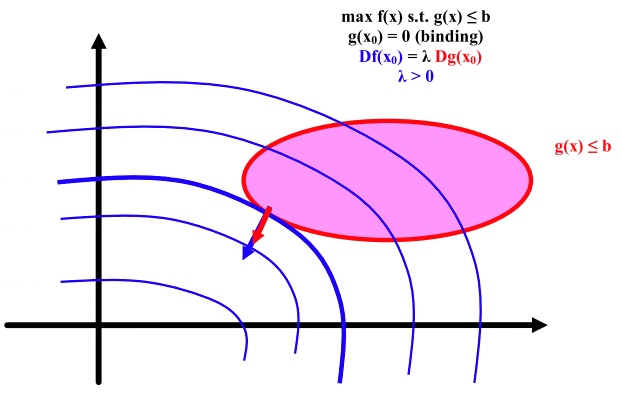
\includegraphics[width=\linewidth]{figs/binding.png}
\caption{Binding constraint}
\end{subfigure}
\begin{subfigure}[b]{0.4\linewidth}
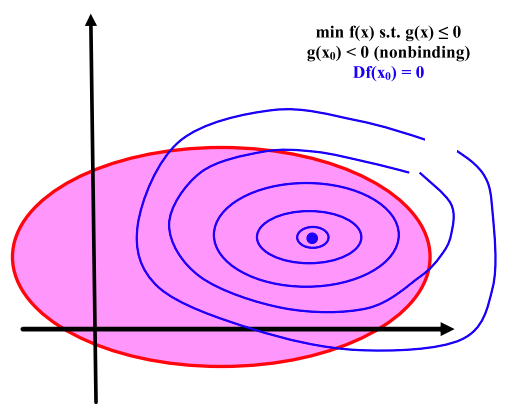
\includegraphics[width=\linewidth]{figs/nonbinding.png}
\caption{Non-binding constraint}
\end{subfigure}
\caption{Constraint binding and non-binding cases}
\end{figure}
	
	\subsection{KKT First-order Conditions for MIN}
	For a minimization problem, you have 3 options
	\begin{enumerate}
		\item \textbf{\red{Flip the sign of the objective function}}, then we will turn a Minimization problem into a Maximization problem, and its FOCs follow suit.
		\item Keep the constraints as is (where all constraints are $\leq$), and the FOCs are the same as the MAXIMIZATION problem \textbf{\red{except that $\lambda \leq 0$}}.
		\item Flip the \textbf{\red{signs of the constraints so that they have the form $\geq$}}, then the FOCs are the same as the MAXIMIZATION problem where $\lambda \geq 0$.
	\end{enumerate}
	
	It is easier to follow the last option.
	\begin{example} \label{example:kkt1}
		\begin{align*}
			\min f(x,y) = 2y - x^2  \\
			s.t. \  x^2 + y^2 \leq 1
		\end{align*}
		Rewrite the problem as
		\begin{align*}
			\min f(x,y) = 2y - x^2  \\
			s.t. \  - x^2 - y^2 \geq -1
		\end{align*}
		The Lagrangian is
		\begin{align*}
			L(x,y,\lambda) = 2y - x^2 - \lambda (-x^2 - y^2 + 1)
		\end{align*}
		FOCs:
		\begin{align*}
			&(i) \ \frac{\partial L}{\partial x} = 0 \iff -2x + 2\lambda x = 0 \\
			&(ii) \ \frac{\partial L}{\partial y} = 0 \iff 2 + 2\lambda y = 0 \\
			&(iii) \ \lambda \cdot (- x^2 - y^2  +1) = 0, \\
			&(iv) \ \lambda \geq 0  \text{ (if $\lambda > 0$, constraint binds).}
		\end{align*}
		From $(i), (ii)$, we can derive $\lambda = 1, y = -1$. Since $\lambda > 0$, the constraint binds and we have $x^2 + y^2 = 1$. Since $y=-1$, we have $x=0$, as the optimum.
	\end{example}
	
		\subsection{Multiple Inequality Constraints}
	Consider an optimization problem of $n$ choice variables and $m$ inequality constraints
	\begin{align}
		\max &f\underbrace{(x_1, \dots, x_n)}_{\x} \label{eq:kkt_prob} &                                                          \\
		s.t. &g_1 (\x) \leq c_1, \nonumber &                                                          \\
		& \dots, \nonumber                                         \\
		& g_m (\x) \leq c_m \nonumber                              
	\end{align}
	
	\begin{ftheorem}[KKT Formulation]
		Steps in solving the problem \eqref{eq:kkt_prob}
		\begin{enumerate}
			\item Write down the Lagrangian
			\begin{align*}
				\mathcal{L}(\x) = f(\x) - \sum_{j=1}^m \lambda_j (g_j(\x) - c_j) 
			\end{align*} 
			
			\item FOCs:
			\begin{align*}
				\frac{\partial \mathcal{L}}{\partial x_i} = 0, \\
			\end{align*}
			for each $i=1, \dots, n$.
			
			\item Complementary slackness
			\begin{align*}
				\lambda_j \geq 0, g_j(\x) = c_j             
				\textbf{ or } \lambda_j = 0, g_j(\x) < c_j 
			\end{align*}
			for $j=1,\dots,m$. Can also be summarized as
			\begin{align*}
				\lambda_j \cdot g_j(\x) = 0.
			\end{align*}	
			
			\item Find all $\x = (x_1,\dots, x_n)$ associated with their $\lambda_1, \dots, \lambda_m$ that satisfy FOCs and the complementary slackness. These are the solution candidates, and at least 1 of them solves the problem if it has a solution.
		\end{enumerate}
	\end{ftheorem}
			\begin{example}
		The problem is
		\begin{align*}
			\max & \ x + 3y - 4 e^{-x-y} \\
			s.t. & \begin{cases}         
				2 - x \geq 2y \\
				x-1 \leq -y
			\end{cases}
		\end{align*}
		Write the problem as
		\begin{align*}
			\max & \ x + 3y - 4 e^{-x-y} \\
			s.t. & \begin{cases}         
				x + 2y \leq 2 \\
				x-1 \leq -y
			\end{cases}
		\end{align*}
		The Lagrangian is
		\begin{align*}
			\mathcal{L}(x,y) = x + 3y - 4 e^{-x-y} - \lambda_1 (x + 2y - 2) - \lambda_2 (x+y-1) 
		\end{align*}
		KKT conditions
		\begin{align*}
			& (i) \ \mathcal{L}'_x = 1 + 4e^{-x-y} - \lambda_1 - \lambda_2 = 0,   \\
			& (ii) \ \mathcal{L}'_y = 3 + 4e^{-x-y} - 2\lambda_1 - \lambda_2 = 0, \\
			&   \lambda_1 \cdot (x+2y-2) = 0, \\
			& \lambda_2 \cdot (x-1+y) = 0, \\
			& (iii) \ \lambda_1 \geq 0 \ (\lambda_1 = 0 \iff x + 2y < 2),         \\
			& (iv) \ \lambda_2 \geq 0 \ (\lambda_2 = 0 \iff x + y < 1)            
		\end{align*}
		Since $\mathcal{L}$ is concave, the KKT conditions are both necessary and sufficient for optimality.
		
		From (ii), (i), we get $\lambda_1 = 2 > 0$, thus making (iii) binds such that $x+2y=2$. Suppose $\lambda_2=0$, there is a contradiction. Suppose $\lambda_2 > 0$, from $(iv)$ we deduce $x+y=1$. Using (i) and (ii), we can find $\lambda_2 = e^{-1} (4-e) > 0$. Thus, the solution is
		\begin{align*}
			(x^*, y^*, \lambda_1, \lambda_2) = (0, \ 1, 2\ , \ e^{-1}. (4-e)) 
		\end{align*}
	\end{example}


		\subsection{Nonnegativity Constraints}
	
	Most oftentimes, in economics, we want to restrict the choice variables to take nonnegative values.
	
	\begin{ftheorem}[Reduced KKT conditions for Nonnegativity]
			Consider the problem
		\begin{align*}
			\max &\ f(x,y)                \\
			s.t. \ & g(x,y) \leq c,                 \\
			& x \geq 0,      \\
			& y \geq 0       
		\end{align*}
		Rewrite the problem to
		\begin{align*}
			\max &f(x,y)                 \\
			s.t. & g(x,y) \leq c,                 \\
			& -x \leq 0,     \\
			& -y \leq 0      
		\end{align*}
		The Lagrangian is \footnote{tips: You should denote the Lagrangian multipliers for the main constraint by $\lambda$ and nonnegativity constraints by $\mu$ for easier handling.}
		\begin{align*}
			\mathcal{L} (x,y) = f(x,y) - \lambda [ g(x,y) - c] - \mu_1 (-x) - \mu_1 (-y) 
		\end{align*}
		The KKT conditions
		\begin{align*}
			& (i) \ \mathcal{L}'_x = f'_x - \lambda g'_x + \mu_1 = 0                       \\
			& (ii) \ \mathcal{L}'_y = f'_y - \lambda g'_y + \mu_2 = 0                      \\
			& (iii) \ \lambda \geq 0, \text{ with } \lambda = 0 \ \text{ if } \ g(x,y) < c \\
			& (iv) \ \mu_1 \geq 0, \text{ with } \mu_1 = 0 \ \text{ if } \ x > 0           \\
			& (v) \ \mu_2 \geq 0, \text{ with } \mu_2 = 0 \ \text{ if } \ y > 0            
		\end{align*}
		Combining (i) and (iv) yields
		\begin{align*}
			f'_x - \lambda g'_x \leq 0, \textbf{ with equality if $x>0$} 
		\end{align*} 
		Combining (ii) and (v) yields
		\begin{align*}
			f'_y - \lambda g'_y \leq 0, \textbf{ with equality if $y>0$} 
		\end{align*} 
		So the KKT conditions are reduced to just
		\begin{align*}
			& f'_x - \lambda g'_x \leq 0, \textbf{ with equality if $x>0$}         \\
			& f'_y - \lambda g'_y \leq 0, \textbf{ with equality if $y>0$}         \\
			& \lambda \geq 0, \text{ with } \lambda = 0 \ \text{ if } \ g(x,y) < c 
		\end{align*}
		
	\end{ftheorem}
	
	\subsection{Examples}
	\begin{example} \label{example:kkt2}
		Consider the utility maximization problem where there are 2 goods $x,y$, price of good $x$ is $p$ and price of good $y$ is normalized to 1, the budget is $m$. Find the optimal $x,y$.
		\begin{align*}
			\max \ & x + \ln(1+y)                                         \\
			s.t. &\ px + y \leq m, \\
			& x \geq 0 \\
			& y \geq 0.                                      
		\end{align*}
		\textbf{Solutions:}
		The Lagrangian is
		\begin{align*}
			L = x + \ln(1+y) - \lambda (px + y - m)
		\end{align*}
		Assume the solution $(x^*,y^*)$ exists, it must satisfy the following KKT conditions
		\begin{align*}
			&(i) & L'_x = 1 - p \lambda \leq 0, \textbf{ with }  1- p\lambda = 0 \iff x^* > 0,  \\
			&(ii) & L'_y = \frac{1}{1+y^*} -\lambda \leq 0 \textbf{ with } \frac{1}{1+y^*} = 0 \iff y^* > 0 \\
			&(iii) & \lambda \cdot (px^* + y^* - m) = 0, \\
			& (iv) & \lambda \geq 0, px^* + y^* \leq m
		\end{align*}
		The objective function is concave in $(x,y)$, the constraint is linear, thus the Lagrangian is concave, so the FOC is also sufficient.
		
		Observe from condition $(i)$ that $\lambda$ cannot be zero, then condition $(iii)$ implies that $\lambda > 0$ and the constraint binds such that
		\begin{align*}
			(iv) \  px^* + y^* = m
		\end{align*}
		Regarding which constraints $x\geq 0, y \geq 0$ bind, we need to consider 4 cases
		\begin{enumerate}
			\item $x^*=0, y^* = 0$: Since $m>0$, this is impossible.
			\item $x^* > 0, y^* = 0$: From $(ii)$, we get $\lambda \geq 1$, then $(i)$ implies that
			\begin{align*}
				p = \frac{1}{\lambda} \leq 1
			\end{align*}
			Then from $(iv)$, we have
			\begin{align*}
				x^* = m/p, \\
				\lambda = 1/p
			\end{align*}	
			if $0 < p < 1$.
			\item $x^* = 0, y^* > 0$: By $(iv)$, we have 
			\begin{align*}
				y^* = m
			\end{align*}
			Then $(ii)$ yields 
			\begin{align*}
				\lambda = \frac{1}{1+y^*} = \frac{1}{1+m}
			\end{align*}
			Then from $(i)$ we get the condition for this is that
			\begin{align*}
				p \geq m+1
			\end{align*}
			\item $x^* > 0, y^* > 0$: With equality in both $(i)$ and $(ii)$, we have
			\begin{align*}
				\lambda = 1/p = 1/(1+y^*)
			\end{align*}
			It follows that
			\begin{align*}
				&y^* = p - 1, \\
				&p > 1 \text{ ( because $y^* > 0$)}
			\end{align*}
			Equation $(iv)$ yields
			\begin{align*}
				&x^* = \frac{m+1-p}{p}, \\
				&p < m+1 \text{ ( because $x^* > 0$)}
			\end{align*}
		\end{enumerate}
		In summary
		\begin{enumerate}
			\item If $0<p \leq 1$, then $(x^*, y^*)  = (m/p, 0)$ with $\lambda = 1/p$ 
			\item if $1<p< m+1$, then $(x^*, y^*) = (\frac{m+1-p}{p}, p-1)$ with $\lambda = 1/p$ 
			\item if $p \geq m+1$, then $(x^*, y^*)  = (0, m)$ with $\lambda = 1/(1+m)$
		\end{enumerate}
		In the 2 extreme cases (1) and (3), it is optimal to spend everything on only the cheaper good -- $x$ in case (1) and $y$ in case (3).
	\end{example}
	
	\subsection{Problem Sets}
	\begin{ex}
		Solve the problem
		\begin{align*}
			&\max  \  f(x,y) = x^2 + y^2 + y - 1, \\
			&s.t. \ g(x,y) = x^2 + y^2 \leq 1 &                             
		\end{align*}
	\end{ex}
	
		\begin{ex}[Cost Function]
		From \citet{varian1992microeconomic}, p.54--58. 
		\begin{enumerate}
			\item Minimizing the cost function for the Cobb-Douglas technology
			\begin{align*}
				\min_{x_1, x_2} &c(\w, y):= w_1 x_1 + w_2 x_2, \\
				\text{ s.t. } &A x_1^\alpha x_2^\beta = y.
			\end{align*}
			Derive the optimal demand for $x_1, x_2$. Let $A=1, \alpha+\beta=1$, find the cost function.
			\item Minimizing the cost function for CES technology
			\begin{align*}
				\min_{x_1, x_2} & w_1 x_1 + w_2 x_2, \\
				\text{ s.t. } & x_1^\rho x_2^\rho = y^\rho.
			\end{align*}
			\item Write the cost function for Leontief technology
			\begin{align*}
				\min_{x_1, x_2} & w_1 x_1 + w_2 x_2, \\
				\text{ s.t. } & f(x_1,x_2) = \min (ax_1, bx_2) = y.
			\end{align*}
			\item Minimizing the cost function for linear technology (using KKT). 
			\begin{align*}
				\min_{x_1, x_2} & w_1 x_1 + w_2 x_2, \\
				\text{ s.t. } & a x_1 + b x_2 = y, \\
				& x_1 \geq 0, \\
				& x_2 \geq 0.
			\end{align*}
		\end{enumerate} 
	\end{ex}
	
	\begin{ex}[Quasilinear Utility]
		From \citet{varian1992microeconomic}, p. 164--165. Solve the problem
		\begin{align*}
			\max_{x_0, x_1} \log(x_1) + x_0, \\
			p_1 x_1 + x_0 = m, \\
			x_0 \geq 0.
		\end{align*}
	\end{ex}
	
	\begin{ex}[Religion] Based on \citet{fan2008religious, farmer2021growth} (p.164). Parents derive utility from consumption, child's future earnings, and religious activities $\rho_t$. Their problem is 
	\begin{align*}
		\max \ln(c_t) + \beta \ln (w_{t+1}) + \zeta \rho_t
	\end{align*} 
	Parents do not work when old and accumulate no physical capital, the constraint is
	\begin{align*}
		c_t = (1-\rho_t) w_t
	\end{align*}
	Human capital is
	\begin{align*}
		h_{t+1} = h_t^\alpha \rho_t^{1-\alpha}.
	\end{align*}
	and wage is determined by human capital
	\begin{align*}
		w_{t+1} = h_{t+1}.
	\end{align*}
	Form the problem such that $\rho_t \geq 0$. 
	\begin{enumerate}
		\item What are the optimal allocations of $c_t, d_{t+1}, \rho_t$?
		\item When will parents not spend time on religious activities?
	\end{enumerate}
	\end{ex}
	
	\begin{ex}[Endogenous Retirement]. 
		In this case, workers are allowed to work in the second period of life \citep{TRAN2022101495}.
		Find the solutions to
		\begin{align*}
			&\max_{c_t, d_{t+1}, l_{t+1}} \ln (c_t) + \pi [ \beta \ln(d_{t+1}) + \gamma \ln(l_{t+1})] \\
			s.t. &\ c_t + s_t = (1-\tau) w_t, \\
			& d_{t+1} = \frac{R_{t+1}}{\pi} s_t + (1-l_{t+1})(1-\tau)\varepsilon w_{t+1} + p_{t+1}l_{t+1} \\
			& l_{t+1} \leq 1 
		\end{align*}
		where $\pi,l_{t+1} \in [0,1]$ are the old-age survival rate, and retirement time portion, $\tau, p$ are social security tax and pension rate. Finally, $\varepsilon \in (0,1)$ is the old-age productivity compared to young-age. The government runs a balanced budget every period such that
		$$
		\tau w_t = p_{t+1}
		$$ 
		\begin{enumerate}
			\item Write the KKT first-order conditions
			\item Derive the Euler equation
			\item Assume that in the equilibrium, $l_{t+1} = 1$ is equivalent to full retirement (individuals do not work in the second period) and $l_{t+1} < 1$ is equivalent to partial retirement (individuals work for a portion of time in the second period), derive a threshold level $\hat{\varepsilon}$ that separates these 2 equilibria.
		\end{enumerate}
		\textbf{Solution:} See Appendix.\ref{AppendixA1}
	\end{ex}
	

	
	\newpage	
	\section{Economic Modeling}
	In previous sections, you have learned how to solve a partial equilibrium problem. That is, we have only considered one part of the equation (household OR firm). In this part, we bring them together in a equilibrium analysis (household AND firm).
	
	\subsection{Endogenous fertility OLG}
		\begin{ex} \label{ex:util1} We first specify the model, solve the problem for each actor inside the model, then bring them together in equilibrium, then study the dynamics of a variable of interest.
	
		\textbf{Household} \\
		A representative household chooses the optimal savings and number of children to maximize their utilities as
		\begin{align*}
			\max_{s_t, n_t} U_t = \ln(c_t) + \beta\ln(R_{t+1} . s_t) + \gamma \ln(n_t),
		\end{align*}
		subject to
		\begin{align*}
			c_t = w_t (1-\phi n_t) - s_t,
		\end{align*}
		given $\beta,\gamma,\phi \in (0,1)$, $w > 0$. 
		\begin{enumerate}
			\item Derive the FOCs that solve the problem for $s_t, n_t$.
			\item Derive $s^*, n^*$ as a function of $w$ and other parameters.
			\item Verify the SOC by checking the signs of the leading minors of the Hessian.
			\item Verify the SOC by evaluating the Eigenvalues of the Hessian.
		\end{enumerate}
		
		\textbf{Firm} \\
		Suppose there is a representative firm of Cobb-Douglas production function
		\begin{align*}
			Y_t = K_t^\alpha L_t^{1-\alpha}
		\end{align*}
		so that its profit is
		\begin{align*}
			\pi_t = p^Y_t Y_t - R_t K_t - w_t L_t
		\end{align*}
		where input prices $R_t, w_t$ are perfectly flexible.
		\begin{enumerate}
			\item Normalize $p^Y_t$ to 1. Derive the optimal $R_t, w_t$ to maximize $\pi_t$.
			\item Let the capital-labor ratio as $k_t = K_t/L_t$, write $w_t, R_t$ in terms of $k_t$.
		\end{enumerate}
		
		\textbf{Dynamics of the Intertemporal Equilibrium} \\
		The dynamics of capital and labor markets are characterized by
		\begin{align*}
			K_{t+1} &= s_t L_t, \\
			L_{t+1} &= L_t (1+n_t).
		\end{align*}
		\begin{enumerate}
			\item Write the law of motion of capital $k_{t+1} \equiv K_{t+1}/L_{t+1}$ in terms of $k_t$. Denote this equation as $k_{t+1} = \phi(k_t)$.
			\item \textbf{[Existence of Equilibria]} Write the difference equation $\triangle k_t \equiv k_{t+1} - g(k_t)$. Show that $\lim_{k_t\to\infty} \triangle k_t$ and $\lim_{k_t\to 0} \triangle k_t$ have opposite signs. In that case, since $\triangle k_t$ is continuous, it must take a value of 0 somewhere, by the Intermediate Value Theorem \citep{de2002theory} (Proposition 1.2, p.20)
			\item \textbf{[Existence of a Steady State]} Show that
			\begin{align*}
				& \text{ (saving is large enough)} \lim_{k\to 0} \frac{k_{t+1}}{k_t} > 1 \text{ or } \lim_{k\to 0} \frac{s_t}{k_t} > 1 + n, \\
				& \text{ (capital is bounded)} \lim_{k\to \infty} f'(k_t) = 0
			\end{align*}
			Also known as ``Absence of Catching Point (Poverty Trap)'' \citep{de2002theory} (Proposition 1.7, p.36), or Inada conditions.
			\item \textbf{[Uniqueness of the Steady State]} Show that for all $k>0$
			\begin{align*}
				\phi'(k_t) > 0, && \phi''(k_t) < 0
			\end{align*}
			\citet{de2002theory} (Proposition 1.3, p.24) requires only the first condition (necessary) while \citet{galor1989existence} demands the second condition for sufficiency. Why unique? [Hint: monotone]
			
			\item Find the steady state $k^*$ by setting $k_{t+1} = k_t = k^*$
			\item \textbf{[Local Stability]} The steady state is locally stable if
			\begin{align*}
				\left| \phi'(k^*) \right| < 1
			\end{align*}
			It is unstable if $\left| \phi'(k^*) \right| > 1$. If it equals 1, then the stability cannot be stated from the first-order derivative basis \citep{de2002theory} (p.42).
			\item Write a code in Python or MATLAB to simulate the model. Use the following parameters $\beta=.99^{120},\gamma=.271,\phi=.15,\alpha=0.3, K_0=L_0=1$. What are the fertility rate, saving rate, and steady-state capital? What will happen to $k^*$ when $\phi$ increases?
		\end{enumerate}
		
		\begin{remark}
			\begin{enumerate}
				\item The SOC check in the Household problem would be unnecessary if the constraints are linear in the choice variables \citep{de2012fertility} (p.26).
				\item Normally, if you assume a Cobb-Douglas production function and a log utility function, the existence and uniqueness, and stability of a non-trivial steady state are (mostly) guaranteed.
				\item In the ``Existence of a Steady State", these conditions are known as strengthened Inada condition \citep{galor1989existence}. The original Inada conditions are stated in the Solow model where
				\begin{align*}
					\lim_{k\to 0} f'(k_t) = \infty, && \lim_{k\to\infty} f'(k_t) = 0.
				\end{align*}
			\end{enumerate}
		\end{remark}
		
	\textbf{Solutions:} See Appendix.\ref{appendix:olg}. 	
	\end{ex}
	

	\subsection{Endogenous education OLG (Beckerian)}
	\begin{ex}
		We modify Exercise \ref{ex:ferti} and use some assumptions from \citet{hirazawa2017labor}. In particular, we bring the model into a general equilibrium framework.
		
	The Household sector is
	\begin{align*}
			\max_{c_t, d_{t+1}, n_t, e_t} & \ln(c_t) + \beta \ln (d_{t+1}) + \gamma \ln ( n_t) + \gamma \ln (\theta + e_t) \\
			\text{s.t.}\ & c_t + s_t + e_t n_t w_t = (1-\phi n_t) w_t h_t, \\
			& d_{t+1} = (1+r_{t+1}) s_t, \\
			& h_{t+1} = 1 + \mu e_t^\eta
		\end{align*}
	where $\alpha,\beta,\gamma,\phi,\eta \in (0,1)$.
	Assume that the production sector has the form
	\begin{align*}
		Y_t = K_t^\alpha L_t^{1-\alpha}
	\end{align*}
	where $L_t = N_t h_t$ is the labor in efficiency units.
	
	\begin{enumerate}
		\item Find the optimal solutions for Households and the representative firm.
		\item Find the changes in $n_t, e_t$ when $w_t$ changes. 
		\item Can $e_t = 0$? Why?
		\item Assume an interior solution for $e_t$, work out the dynamics of $k_t$ and $h_t$.
		\item Find the steady states of $k$ and $h$ (if possible).
		\item Change the human capital accumulation function to $h_{t+1} = \mu e_t^\eta h_t^{1-\eta}$ and see if the problems can be solved more easily.
	\end{enumerate}
	
	\begin{remark}
		At this point, an usual procedure is to analyze the stability of this steady state. However, since there are 2 dynamic variables $k_{t+1}$ and $h_{t+1}$, stability analysis can be difficult. The idea is still the same, we want to show that the ``derivatives" of the future variable wrt the current variable be smaller than 1. However, for a system of 2 dynamic equations of 2 variables, we need to rely on the Jacobian. The idea is implemented in the following exercise \ref{ex:dynamic}.
	\end{remark}
	\end{ex}
	
	\begin{ex}[Inter-generational Taste Externalities]
		\label{ex:dynamic} This exercise is from \citet{de2002theory} p.248, which is a simplified version of \citet{de1996dynamics}. Consider the following utility function
		\begin{align*}
			U_t = \ln(c_t - \theta a_t ) + \beta \ln(d_{t+1})
		\end{align*}
		where $\theta \in (0,1)$ measure the intensity of inter-generational spillover (aspiration). And
		\begin{align*}
			\text{ (habit formation) } & a_t = c_{t-1}, \\
			\text{ (budget constraint) } & c_t + s_t = w_t.
		\end{align*}
		\begin{enumerate}
			\item Find the solution for the saving function.
			\item Assume that the production function is Cobb-Douglas where $f(k_t) = A k_t^\alpha$. Find the competitive wage and interest rate.
			\item Assume $k_{t+1} = s_t$. Write the system of 2 dynamic equations $k_{t+1} = \phi (k_t, a_t)$ and $a_{t+1} = \psi (k_t, a_t)$. Find their steady states $\bar{k}, \bar{a}$.
			\item Under what conditions the steady states are locally stable?
		\end{enumerate}
	\end{ex}
		
	%===================== Dyn Opt ====================%
	
	\chapter{Dynamic Optimization}
	There are 2 versions of dynamic optimization methods. The first deals with continuous time, where a variable is differentiable with time. The second deals with discrete time, where a variable is not differentiable with respect to time.
	
	\begin{figure}[h!]
\centering
\begin{subfigure}[b]{0.45\linewidth}
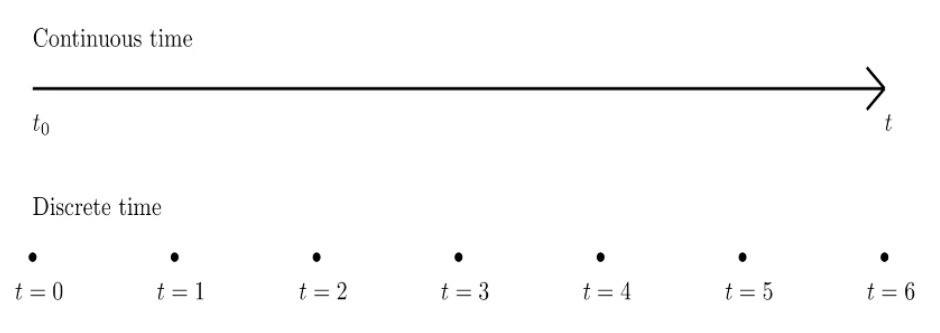
\includegraphics[width=\linewidth]{figs/concept1.png}
%\caption{Coffee.}
\end{subfigure}
\begin{subfigure}[b]{0.45\linewidth}
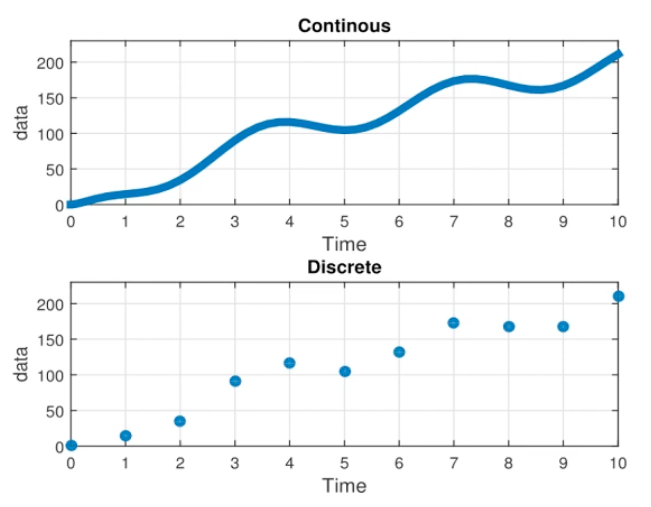
\includegraphics[width=\linewidth]{figs/concept2.png}
%\caption{More coffee.}
\end{subfigure}
\caption{Conceptualization of Time. Source: \href{https://www.youtube.com/watch?v=w9VM7is9cl8}{Klaus Prettner}}
\label{fig:concept}
\end{figure}

	
	\section{Dynamic Programming}
	Also known as Discrete-Time Optimization. Household solves
	\begin{align*}
		\max_{c_t} & \sum^\infty_{t=0} \beta^t u(c_t), \\
		s.t. &\ c_t = f(k_t) - k_{t+1} + (1-\delta) k_t.
	\end{align*}
	Assume a nonzero initial condition, the constraint gives us the equation of motion of the state variable
	\begin{align*}
		&(\textbf{transition equation}) & k_{t+1} &= f(k_t) + (1-\delta)k_t - c_t, \\
		&(\textbf{initial condition}) & k_0 &> 0
	\end{align*}
	Find the solution for the optimal choice of $c_t$.
	
	\subsection{Lagrangian Method}
	The Lagrangian:

$$
    \mathcal{L} = \sum_{t=0}^{\infty} \beta^t u(c_t) + \sum_{t=0}^{\infty} \lambda_t \left[ f(k_t) + (1- \delta) k_t - k_{t+1} - c_t \right]
$$

Grouping all the summation and rewriting the Lagrangian:
$$
    \mathcal{L} = \sum_{t=0}^{\infty} \left[ \beta^t u(c_t) + \lambda_t \left( f(k_t) + (1- \delta)k_t - k_{t+1} - c_t \right) \right]
$$

The term inside the sum should be optimized at each point in time. The modified Lagrangian:
$$
    L = \beta^t u(c_t) + \lambda_t \left( f(k_t) + (1- \delta) k_t - k_{t+1} - c_t \right)
$$

FOC: (Note that $k_{t+1}$ appears twice at time $t$ and $t+1$)

\begin{align}
      &(c_t): \frac{\partial L}{\partial c_t} = \beta^t u'(c_t) - \lambda_t = 0  \label{eq:foc_c}  \ \                                                \\
      &(k_{t+1}): \frac{\partial L}{\partial k_{t+1}} = -\lambda_t + \lambda_{t+1} \left[ f'(k_{t+1}) + (1-\delta) \right] = 0 \label{eq:foc_k} \ 
\end{align}

By virtue of Eq.~\eqref{eq:foc_c}, we see that:

$$
    \beta^{t+1}u'(c_{t+1}) = \lambda_{t+1}
$$

Plugging back to Eq.~\eqref{eq:foc_k} and rearranging give us the Euler equation:

$$
    \frac{u'(c_t)}{u'(c_{t+1})} = \beta \left[ f'(k_{t+1}) + (1-\delta) \right]
$$

Consider the utility function $u(c_t) = \ln(c_t)$, we have:

$$
    \frac{c_{t+1}}{c_t} = \beta \left[f'(k_{t+1}) + (1-\delta)\right]
$$

In the steady-state, $c_{t+1} = c_t = \bar{c}$ and $k_{t+1} = k_t = \bar{k}$.  

Provided with a functional form of the production function $f(k)$, one can find the steady-state values of $\bar{c}, \bar{k}$ and then use backward induction to figure out the dynamics from a given $k_0$.
	
	\subsection{Bellman Method}
	The following steps describe Bellman's method.
	\begin{enumerate}
		\item Set up the Bellman equation
		\begin{align*}
			V(k_t) = \max \left[ u(c_t) + \beta V(k_{t+1}) \right]
		\end{align*}
		where one can replace
		\begin{align*}
			c_t = f(k_t) - k_{t+1} + (1-\delta) k_t
		\end{align*}
		so the problem changes from optimizing $c_t$ to optimizing $k_{t+1}$. Let's rewrite the Value Function as
		\begin{align*}
			V(k_t) = \max_{k_{t+1}} \left[ u(f(k_t) - k_{t+1} + (1-\delta)k_t) +\beta V(k_{t+1}) \right] 
		\end{align*}
		\item Maximizing the Value function wrt. the control variable $k_{t+1}$:
		\begin{align*}
			\frac{\partial V(k_t)}{\partial k_{t+1}} = 0 \Leftrightarrow \frac{\partial u(k_{t+1})}{\partial k_{t+1}} + \beta \blue{\frac{\partial V(k_{t+1})}{\partial k_{t+1}}} = 0 
		\end{align*}
		\item Do we know $\blue{\frac{\partial V(k_{t+1})}{\partial k_{t+1}}}$? Yes, it can be obtained by differentiating the Value Function to the state variable $k_t$
		\begin{align*}
			\frac{\partial V(k_t)}{\partial k_t} = (f'(k_t) + 1-\delta) u'( f(k_t) - k_{t+1} + (1-\delta)k_t ) 
		\end{align*}
		implying that
		\begin{align*}
			\frac{\partial V(k_{t+1})}{\partial k_{t+1}} &= (f'(k_{t+1}) + 1-\delta) u'\red{( f(k_{t+1}) - k_{t+2} + (1-\delta)k_{t+1} )} \\
			&= (f'(k_{t+1}) + 1-\delta)u'\red{ (c_{t+1})}
		\end{align*}
		\item Derive the Euler equation relating the dynamics of the choice variable.
		\begin{align*}
			\frac{u'(c_t)}{u'(c_{t+1})} = \beta (f'(k_{t+1}) + (1-\delta))
		\end{align*}
		where the transversality condition holds
		\begin{align*}
			\lim_{t\to 0} \beta^t u'(c_t) k_{t+1} = 0.
		\end{align*}
	\end{enumerate}


	
	\section{Optimal Control}
	Also known as Continuous-Time Optimization. Let us consider the problem
	\begin{align}
		\max_{ \{c_t\}^T_{t=0} } e^{-(\rho-n) t} u(c_t)  dt, \\
		s.t. \ c_t + \dot{k}_t = f(k_t) - \delta k_t.
	\end{align}
	The control variable is $c_t$ and the state variable is $a_t$. Assume a nonzero initial condition, the constraint gives us the equation of motion for the state variable
	\begin{align*}
		&(\textbf{transition equation}) & \dot{k}_t &= f(k_t) - \delta k_t - c_t, \\
		&(\textbf{initial condition}) & k_0 &> 0
	\end{align*}

	
	\subsection{Lagrangian Method}
	Everything begins with the Lagrangian function. In fact, it's more intuitive to start here than going straight to Hamiltonian:

$$
    \mathcal{L} = \int_{0}^{\infty} e^{-\rho t} u(c(t)) dt + \int_{0}^{\infty} \lambda(t) \left[ f( k(t)) - \delta k(t) - c(t) - \dot{k}(t) \right] dt
$$

It's the sum of 2 integrals with the same boundary and the same variables (time), so we can sum them up and rewrite the Lagrangian:

$$
    \mathcal{L} = \int_{0}^{\infty} \left\{ e^{-\rho t} u(c(t)) + \lambda(t) \left[ f( k(t)) - \delta k(t) - c(t) - \dot{k}(t) \right] \right\} dt
$$

We want to maximize $c(t)$ with respect to $k(t)$, but $\dot{k}(t)$ is not independent with $k(t)$. So $\dot{k}(t)$ needs to be got rid of, and can somehow be expressed in terms of $k(t)$.

First, separate the $\dot{k}(t)$ term out of the integral.

$$
    \mathcal{L} = \int_{0}^{\infty} \left\{ e^{-\rho t} u(c(t)) + \lambda(t) \left[ F( k(t)) - \delta k(t) - c(t)  \right] \right\} dt - \int_{0}^{\infty} \lambda(t)\dot{k}(t)dt
$$

Using integration by parts  for the second integral term:

$$
     \int_{0}^{\infty} \lambda(t) \dot{k}(t) dt                                               \\
     = \lambda(t) k(t) \Big|_0^\infty - \int_{0}^{\infty} \dot{\lambda}(t)k(t)dt              \\
     = \lambda(\infty) k(\infty) - \lambda(0) k(0) - \int_{0}^{\infty} \dot{\lambda}(t)k(t)dt 
$$

Notice that if $k$ at time $t=\infty$ is indeed $\infty$, and $\lambda(\infty)$ (the penalty term) is also non-zero, then there is no reason to consume now. The household will wait until the very very end of time close to infinity since the utility is essentially infinity. On the other hand, if $k$ at $t=\infty$ is $-\infty$, there is no reason to save, it's better to consume everything and leave nothing left. Such extreme cases would appear if $\lambda(\infty)k(\infty)$ is not bounded and it will dominate everything.

To counter that problem, we introduce the transversality (no Ponzi scheme) condition.

$$
    \lim_{t\to\infty} \lambda(t)k(t) = 0
$$

We also assume $k(0)$ is given and is a constant (the economy needs something to start with), meaning it will disappear when we derive the FOC. As it is given, there should be no penalty term ($\lambda(0) = 0$). Thus, we have:

$$
    \int_{0}^{\infty} \lambda(t)\dot{k}(t) dt = - \int_{0}^{\infty} \dot{\lambda}(t) k(t) dt
$$

Plugging back to the Lagrangian $\mathcal{L}$, we obtain:

$$
    \mathcal{L} = \int_{0}^{\infty} \left\{ e^{-\rho t} u(c(t)) + \lambda(t) \left[ F( k(t)) - \delta k(t) - c(t)  \right] \right\} dt + \int_{0}^{\infty} \dot{\lambda}(t)k(t)dt 
$$

Sum them back to under 1 integral again:

$$
    \mathcal{L} = \int_{0}^{\infty} \left\{ e^{-\rho t} u(c(t)) + \lambda(t) \left[ F( k(t)) - \delta k(t) - c(t)  \right] +  \dot{\lambda}(t)k(t) \right\} dt 
$$

The Lagrangian enables us to maximize the function at each point in time, so we only care about maximizing the functional form inside the integral (we don't care about time anymore). Rewrite the term inside the integral as $L$, and call this the *modified Lagrangian*. The following 2 expressions are equivalent.

\begin{align}
     L = {e^{-\rho t} u(c(t)) + \lambda(t) \left[ f( k(t)) - \delta k(t) - c(t)  \right]} -  \lambda(t)\dot{k}(t)     \label{eq:foc_c2} \\                            
     L =  \underbrace{e^{-\rho t} u(c(t)) + \lambda(t) \left[ f( k(t)) - \delta k(t) - c(t)  \right]}_{\text{Hamiltonian}}+  \dot{\lambda}(t)k(t)  \label{eq:foc_k2}
\end{align}

Terminologically speaking: $c(t)$ is the control variable since it can jump (taking any value at any point in time) while $k(t)$ is the state variable because it accumulates over time. ${\lambda}(t)$ is the co-state variable (also known as *shadow price* in economics because it shows the marginal cost of violating the constraints at each point in time). 

Sticking with the Lagrangian method, we derive the FOC:

\begin{align}
     &(c(t)): \frac{dL}{d c(t)} = e^{-\rho t} u'(c(t)) - \lambda(t) = 0  \text{(using \eqref{eq:foc_c2})}     \\   
     &(k(t)): \frac{dL}{d k(t)} = \lambda(t) [ f'(k(t)) - \delta] + \dot{\lambda}(t) = 0 \ \text{(using Eq.\eqref{eq:foc_k2})} \\
     &(\lambda(t)): \frac{dL}{d \lambda(t)} = f(k(t)) - \delta k(t) - c(t) = 0 \ \text{(using \eqref{eq:foc_c2})}           
\end{align}

We need to get rid of $\lambda$. From $(c(t))$ condition, we derive:

$$
    \lambda(t) = e^{-\rho t} u'(c(t))
$$

Thus, $\dot{\lambda}(t)$ can be derived as:

$$
    \dot{\lambda}(t) = \frac{d \lambda(t)}{dt} = -\rho e^{-\rho t} u'(c(t)) + e^{-\rho t} u''(c(t)) \dot{c}(t)
$$

And we obtain:

$$
    \frac{\dot{\lambda}(t)}{\lambda(t)} = -\rho \frac{u'(c(t))}{u'(c(t))} + \frac{u''(c(t))}{u'(c(t))}\dot{c}(t) = - \rho + \frac{u''(c(t))}{u'(c(t))}\dot{c}(t)
$$

We can explicitly derive the condition for a functional form of $u$, especially with CRRA (constant relative risk aversion). For simplicity, let $u(c) = \ln(c)$, then $u'(c(t)) = \frac{1}{c(t)}$ and $u''(c(t)) = \frac{-1}{c^2(t)}$. Plugging back into the above equation, we obtain:

$$
    \frac{\dot{\lambda}(t)}{\lambda(t)} = -\rho - \frac{\dot{c}(t)}{c(t)} \ \ (5)
$$

From the FOC of $k(t)$, we know that:

$$
    - \frac{\dot{\lambda}(t)}{\lambda(t)} = f'(k(t)) - \delta
$$

Combining with Eq. (5) yields the Euler equation:

$$
\frac{\dot{c}(t)}{c(t)} = f'(k(t)) - \delta -\rho
$$

This condition constitutes the optimal path of consumption chosen by the household.

	\subsection{Hamiltonian}
	A cookbook method (Pontryagin’s maximum principle) for this problem.
		The maximum principle can be summarized as a series of steps with the economic intuition explained as follows \citep{campante2021advanced}.
	\begin{enumerate}
		\item Set at the present-value Hamiltonian
		\begin{align}
			H_t = u(c_t)e^{-\rho t} + \lambda_t ( \underbrace{f(k_t) - c_t - \delta k_t}_{\dot{k}_t})
		\end{align}
		where $\lambda_t$ is called the co-state variable. The Hamiltonian is similar to the way you obtain the Lagrangian (but without integral). The interpretation of the co-state variable $\lambda_t$ is the same as the Lagrangian multiplier. It tells you the marginal benefit of a marginal addition to the stock of the state variable $k_t$ (in economic jargon, it is called ``the shadow value/ price of the state variable"), which is also the value of the state variable at $t=0$.
				
		\item Take the FOC of Hamiltonian wrt the control variable(s)
		\begin{align}
			\frac{\partial H_t}{\partial c_t} = 0 \Leftrightarrow e^{-\rho t} u'(c_t) = \lambda_t. \label{eq:hc}
		\end{align}
		This is legitimate since the Hamiltonian is static at each $t$, so the optimal value of the choice variable should be done in a static optimization fashion. \eqref{eq:hc} states that the marginal utility gain from increasing consumption has to be equal to the marginal cost ($\lambda$) of not adding such amount to the stock of your assets (the state variable).
		
		\item Derive the optimal path of the state and co-state variable(s)
		\begin{align}
			\dot{k}_t &= \frac{\partial H_t}{\partial \lambda_t} = f(k_t) - c_t - \delta k_t, \label{eq:kdot} \\
			\dot{\lambda}_t &= \red{-} \frac{\partial H_t}{\partial k_t} = - \lambda_t (f'(k_t) - \delta) \label{eq:costate}
		\end{align}
		The Hamilton is static, but our model is dynamic. This means that, at any instant, we must figure out that whatever we leave for the next instant is consistent with optimization. This is the key insight into the problem. Furthermore, what we care about in an infinite time span can be broken down into a sequence of choices between the current instant and the next in an infinitesimally small time frame.
		
		To figure out that path, the maximization principle tells you that you need to satisfy the co-state equations. The first equation \eqref{eq:kdot} links one instant of the state variable to the next and must be satisfied at any time. The second equation \eqref{eq:costate} is an ``asset pricing" condition. Basically, the term $\dot{\lambda}_t$ is the appreciation in the marginal value of capital, so $-\dot{\lambda}_t$ is its depreciation. If you carry more capital to the next, its value should depreciate more as the volume increase. The term $\partial H/\partial k$, on the other hand, shows the marginal return of capital at this instant, contributing to the utility and production (which are encompassed in the Hamiltonian). Obviously, the equilibrium is brought by equalizing the 2 terms. (\href{https://www3.nd.edu/~nmark/Climate/CurrentValueHamiltonian.pdf}{Read more})
		
		\item Set the transversality condition
		\begin{align}
			\lim_{t\to\infty} \lambda_t k_t = 0. \label{eq:trans}
		\end{align}
		While the transition \eqref{eq:kdot}, and Euler equations (\eqref{eq:hc}, \eqref{eq:costate}) jointly govern the temporal behavior of consumption and capital (state variable), the initial and transversality conditions specify the state of the economy at the boundaries (i.e., $t = 0$ and $t = \infty$). Initially, the economy must start with something it can work with -- $k_0 > 0$. The transversality condition, in particular, prevents the over-accumulation of capital by requiring zero present value of the capital in an infinitely distant future. 
		
		In a finite time horizon (i.e., you must die at some point $T$), it makes sense that $\lambda(T) = 0$, so you have no incentive to save for the next period, you must consume everything. However, things get more complicated as we progress to the infinite horizon. Without this equation, households will keep accumulating capital indefinitely as capital has value $\lambda$ and households still have $k_t$ in expense, which implies that a steady state cannot be secured. To prevent this case from happening, condition \eqref{eq:trans} is necessary. The requirement is that at the limit $t\to\infty$, if the terminal capital has a positive present value, then you must consume it all to make $k(t) = 0$. Otherwise, it must have zero valuation $\lambda_t$ so that you are indifferent about leaving it unexploited. This transversality condition that imposes a non-negativity constraint on capital is also known as the ``no-Ponzi scheme" condition
		
		\item Derive the Euler equation relating the dynamics of the choice variable
		\begin{align}
			\rho - \frac{u''(c_t) \dot{c}_t}{u'(c_t)} = f'(k_t) - \delta. \label{eq:euler}
		\end{align}
		Ultimately, we are interested in the dynamic behavior of the control and state variable over time. This is done by taking \eqref{eq:hc} and differentiating both sides with respect to time (product and chain rule)
		\begin{align}
			\dot{\lambda}_t = -\rho e^{-\rho t} u'(c_t) + e^{-\rho t} u''(c_t) \dot{c}_t
		\end{align}
		which is the co-state variable. Substituting it to \eqref{eq:costate}, we have
		\begin{align*}
			-\rho e^{-\rho t} u'(c_t) + e^{-\rho t} u''(c_t) \dot{c}_t = -\lambda_t (f'(k_t)-\delta)
		\end{align*}
		and using \eqref{eq:hc} for $\lambda_t$, we obtain
		\begin{align*}
			-\rho e^{-\rho t} u'(c_t) + e^{-\rho t} u''(c_t) \dot{c}_t = - e^{-\rho t} u'(c_t) (f'(k_t)-\delta)
		\end{align*}
		Dividing both sides by $e^{-\rho t} u'(c_t)$, we obtain \eqref{eq:euler}. If we assume a log utility function, then it is easy to obtain the same result with Lagrangian
		\begin{align*}
			\frac{\dot{c}_t}{c_t} = f'(k_t) - \delta - \rho. 
		\end{align*}
	\end{enumerate}
	
	\section{Models}
	
	\subsection{RCK}
	This section deals with the neoclassical growth model, also known as the Ramsey-Cass-Koopsman, in continuous time. \citet{ramsey1928mathematical} first solved this problem before he died at the age of 26. He was so ahead of his time that nearly 4 decades later, by the works of \citet{cass1965optimum} and \citet{koopmans1963concept}, the model became as well-known as today. 
	
	\subsubsection{Endogenous Labor}
	The economy solves
	\begin{align*}
		\max & \int^\infty_0  \beta^t \left[ \ln(c_t) + \gamma \ln(1-l_t)\right] dt, \\
		\text{ s.t. } c_t + i_t &= y_t, \\
		y_t &= f(k_t) = A k_t^\alpha, \\
		\dot{k}_t &= i_t - \delta k_t
	\end{align*}
	
	\subsection{Real Business Cycle}
	
	\subsection{Dynamic General Equilibrium}
		
	\subsection{Continuous-time OLG}
	
	\section{Programing}
	Sources:
	\begin{enumerate}
		\item \url{https://python-advanced.quantecon.org/discrete_dp.html}
		\item \url{https://macroeconomics.github.io/Dynamic%20Programming.html}
		\item \url{https://github.com/lnsongxf/NumEcon/tree/master/numecon/macro}
	\end{enumerate}
	\subsection{Backward Induction}
	\subsection{Value Function Iteration}
	\subsection{Policy Function Iteration}
	
		

	
	
	\addcontentsline{toc}{chapter}{References}
	\bibliography{bibliography.bib}
	
	\begin{appendices}
	
	\chapter{Cheatsheets}
		\section{Differentiation}
	See Chapter 5 of \citet{springcamp}.
	\subsection*{Basic Rules}
	\begin{align*}
		&(cf)' = cf' &&
		&(f+g)' = f' + g' \\
		&(fg)' = f'g + fg' &&
		&(f/g)' = \frac{f'g - fg'}{g^2} \quad (g \neq 0) \\
		&(f \circ g)' = f'(g(x)) \cdot g'(x)
	\end{align*}
	
	\subsection*{Common Derivatives}
	\begin{align*}
		&\frac{d}{dx} (x^n) = nx^{n-1} &&
		&\frac{d}{dx} (e^x) = e^x &&
		&\frac{d}{dx} (\ln x) = \frac{1}{x} &&
		&\frac{d}{dx} \left(\frac{1}{x}\right) = -\frac{1}{x^2}
	\end{align*}
	
	\subsection*{Chain Rule}
	\[
	\frac{d}{dx} (f(g(x))) = f'(g(x)) \cdot g'(x)
	\]
	
	\subsection*{Product Rule}
	\[
	\frac{d}{dx} (uv) = u'v + uv'
	\]
	
	\subsection*{Quotient Rule}
	\[
	\frac{d}{dx} \left( \frac{u}{v} \right) = \frac{u'v - uv'}{v^2} \quad (v \neq 0)
	\]
	
	\subsection*{Power Rule}
	\[
	\frac{d}{dx} (x^n) = nx^{n-1}
	\]
	
	\subsection*{Exponential Rule}
	\[
	\frac{d}{dx} (e^{u(x)}) = u'(x) e^{u(x)}
	\]
	
	\section{Integration}
	See Chapter 8 of \citet{springcamp}
	\subsection*{Basic Integrals}
	\begin{align*}
		&\int k \, dx = kx + C \quad \text{(where $k$ is a constant)} \\
		&\int x^n \, dx = \frac{1}{n+1} x^{n+1} + C \quad \text{(where $n \neq -1$)} \\
		&\int e^x \, dx = e^x + C \\
		&\int \frac{1}{x} \, dx = \ln |x| + C
	\end{align*}
	
	\subsection*{Common Integrals}
	\begin{align*}
		&\int e^{ax} \, dx = \frac{1}{a} e^{ax} + C \\
		&\int \ln x \, dx = x \ln x - x + C
	\end{align*}
	
	\subsection*{Integration by Parts}
	\[
	\int u \, dv = uv - \int v \, du
	\]
	
	\section{Taylor Series Formula}
	See Chapter 6.6 of \citet{springcamp}. The Taylor series expansion of a function $f(x)$ at a point $a$ is given by:
	\[
	f(x) = f(a) + f'(a)(x - a) + \frac{f''(a)}{2!}(x - a)^2 + \frac{f'''(a)}{3!}(x - a)^3 + \dotsb
	\]
	Or, in sigma notation:
	\[
	f(x) = \sum_{n=0}^{\infty} \frac{f^{(n)}(a)}{n!}(x - a)^n
	\]
	\subsection*{Order 1}
	The Taylor series formula of order 1 for a function $f(x)$ centered at $a$ is given by:
	\[
	f(x) = f(a) + f'(a)(x - a)
	\]
	
	\subsection*{Order 2}
	The Taylor series formula of order 2 for a function $f(x)$ centered at $a$ is given by:
	\[
	f(x) = f(a) + f'(a)(x - a) + \frac{f''(a)}{2!}(x - a)^2
	\]
	
	\section{Implicit Function Theorem}
	See Chapter 10.6 of \citet{springcamp}. Let \( F(x, y) \) be a continuously differentiable function defined in a neighborhood of a point \( (a, b) \). If \( F(a, b) = 0 \) and \( \frac{\partial F}{\partial y} \neq 0 \) at \( (a, b) \), then there exists an open interval \( I \) containing \( a \) and an open interval \( J \) containing \( b \), and a unique continuously differentiable function \( f : I \to J \), such that for all \( x \) in \( I \), the equation \( F(x, f(x)) = 0 \) holds.
	
	Furthermore, the derivative \( f'(x) \) where $y = f(x)$ is given by:
	\[ f'(x) = -\dfrac{\dfrac{\partial F}{\partial x}(x, f(x))}{\dfrac{\partial F}{\partial y}(x, f(x))} \]
	
	\red{Sometimes, when explicit solutions are not attainable, you can perform comparative statics with this theorem.} 	
	\begin{example}
		Find $y'(x)$ when $xy=5$.
		
		Let $F(x,y) = xy$. Then $F'_x = y, F'_y = x$. For $x\neq 0$, the IFT says that
		\begin{align*}
			y' = - \frac{F'_x}{F'_y} = - \frac{y}{x} 
		\end{align*}
	\end{example}
	
	
	\section{Intermediate Value Theorem}
	See Chapter 6.10 of \citet{springcamp}. Let \( f \) be a continuous function on the closed interval \([a, b]\). If \( y \) is any number between \( f(a) \) and \( f(b) \), then there exists at least one number \( c \) in the open interval \((a, b)\) such that \( f(c) = y \).
	
	\textbf{Application:} \red{Mostly to prove the existence of a solution.}
	
	We can use the Intermediate Value Theorem (IVT) to show that certain equations have solutions, or that certain polynomials have roots. For instance, the polynomial \( f(x) = x^4 + x - 3 \) is complicated, and finding its roots is very complicated. However, it's easy to check that \( f(-1) = -3 \) and \( f(2) = 15 \). Since \( -3 < 0 < 15 \), there has to be a point \( c \) between -1 and 2 with \( f(c) = 0 \). In other words, \( f(x) \) has a root somewhere between -1 and 2. We don't know where, but we know it exists.
	
	In a more general concept, if you need to solve
	\begin{align*}
		f(x) = g(x)
	\end{align*}
	Sometimes, solving it is difficult. Instead, you can use numerical methods (that is, let the computer do the hard part). However, you may still want to prove the existence of such an $x^*$. Then you can show that $f(x)$ is increasing from $[-\infty,\infty]$, while $g(x)$ is decreasing from $[-\infty,\infty]$. Thus, they must cross somewhere, and that somewhere is $x^*$. And if $f$, $g$ are monotone, then this $x^*$ is unique.
	
	\begin{example}
		Prove that the equation
		$$2x - 5e^{-x}(1+x^2)=0$$
		has a unique solution, which lies in the interval (0, 2).
		
		\textbf{Solution}:
		
		Define $g(x) = 2x - 5e^{-x}(1 + x^2)$. Then $g(0) = -5$ and $g(2) = 4 - 25/e^2$. In fact $g(2) > 0$ because $e > 5/2$. According to the intermediate value theorem, therefore, the continuous function $g$ must have at least one zero in $(0, 2)$. Moreover, note that $g'(x) = 2 + 5e^{-x}(1+x^2)-10xe^{-x} =2+5e^{-x}(1-2x+x^2)=2+5e^{-x}(x-1)^2$.But then $g'(x)>0$ for all $x$, so $g$ is strictly increasing. It follows that $g$ can have only one zero.
	\end{example}
	
	\section{Matrix Algebra}
	See Chapter 9 of \citet{springcamp}
	\subsection{Matrix Operations}
	
	\subsubsection*{Addition and Subtraction}
	\[
	A + B = B + A \quad \text{(Commutative)}
	\]
	\[
	(A + B) + C = A + (B + C) \quad \text{(Associative)}
	\]
	
	\subsubsection*{Scalar Multiplication}
	\[
	c(A + B) = cA + cB
	\]
	\[
	(c + d)A = cA + dA
	\]
	
	\subsubsection*{Matrix Multiplication}
	\[
	A(BC) = (AB)C \quad \text{(Associative)}
	\]
	\[
	A(B + C) = AB + AC \quad \text{(Distributive)}
	\]
	\[
	(cA)B = A(cB) = c(AB)
	\]
	\subsection{Matrix Multiplication}
	
	Given matrices \( A_{m \times p} \) and \( B_{p \times n} \), their matrix product \( C = AB \) is defined by the formula:
	\[
	C_{ij} = \sum_{k=1}^{p} A_{ik} \cdot B_{kj}
	\]
	where \( 1 \leq i \leq m \) and \( 1 \leq j \leq n \).
	
	In other words, the entry in the \( i \)-th row and \( j \)-th column of \( C \) is obtained by multiplying the elements in the \( i \)-th row of \( A \) with the corresponding elements in the \( j \)-th column of \( B \), and then summing up these products.
	
	\subsection{Transpose}
	A transpose $\A^T$ of a $k \times n$ matrix is the $n\times k$ matrix obtained by interchanging rows and columns of $\A$. Notation: $\A^T$ or $\A'$.
	
	\begin{fdefinition}[Rules for Transposition]
		\begin{align*}
			(\A+\B)^T = \A^T + \B^T,    \\
			(\A-\B)^T = \A^T - \B^T,    \\
			(\A^T)^T = \A,              \\
			(r\A)^T = r\A^T,            \\
			\red{(\A\B)^T = \B^T \A^T}. 
		\end{align*}
		A matrix is \textbf{symmetric} iff $\A = \A'$
	\end{fdefinition}
	
	\subsection{Determinants}
	\subsubsection*{Order 2}
	The determinant of a $2\times 2$ matrix is given by
	\begin{align*}
		|\A| = \begin{vmatrix}
			a & b \\ c & d
		\end{vmatrix} = ad - cb
	\end{align*}
	
	\subsubsection*{Order 3}
	The determinant of a $3\times 3$ matrix is given by:
	\begin{align*}
		|A| &= \det \begin{pmatrix}
			a_{11} & a_{12} & a_{13} \\
			a_{21} & a_{22} & a_{23} \\
			a_{31} & a_{32} & a_{33} 
		\end{pmatrix} \\
		%&= a_{11} |C_{11}| + a_{12} |C_{12}| + a_{13} |C_{13}| \\
		%&= a_{11} |M_{11}| - a_{12} |M_{12}| + a_{13} |M_{13}| \\
		&= a_{11} [a_{22}a_{33} - a_{32}a_{23}] 
		- a_{12}[a_{21}a_{33} - a_{31}a_{23}] 
		+ a_{13}[a_{21}a_{32} - a_{31}a_{22}]
	\end{align*}
	For higher order, see the Spring Camp's materials. Most oftentimes, you need the determinant to be nonzero.
	
	\section{Jacobians, Gradients, and Hessians}
	The Gradient $\nabla$ is a vector that points in the direction of the steepest increase of a scalar-valued (1D) function of multiple variables. Its magnitude $|\nabla |$ is the rate of change in that direction. The gradient is a vector and has the same dimension as the number of variables in the function. For a function of $n$ variables, the gradient is an n-dimensional vector.
	
	The Jacobian is a matrix that represents the collection of all first-order partial derivatives of a vector-valued function with respect to multiple variables. It provides information about how each component of the vector function changes as the variables change. The Jacobian is a matrix whose size is determined by the number of components in the vector-valued function and the number of variables. For a function with $m$ components (functions) and $n$ variables, the Jacobian is an $m \times n$ matrix.
	
	In summary, the gradient is a vector that describes the rate of change of a scalar-valued (1D) function, while the Jacobian is a matrix that describes the rate of change of a vector-valued (n-D) function.
	
	The Hessian is just a matrix of second-order mixed partials of a scalar field (that is, gradients). The Hessian matrix is symmetric. This means that the element in row 
	i and column 
	j is the same as the element in row 
	j and column 
	i.
	The mixed partial derivatives in the Hessian matrix satisfy the equality of mixed partials $\frac{\partial^2 f}{\partial x \partial y} = \frac{\partial^2 f}{\partial y\partial x}$. The eigenvalues of the Hessian matrix are indicators of the curvature of the function at a critical point. Positive eigenvalues suggest a local minimum, negative eigenvalues suggest a local maximum, and a mix of positive and negative eigenvalues suggest a saddle point. For more detail, see Chapter 10 of \citet{springcamp}.
	
	\subsection*{1D (1 dimension)}
	Let \( f(x) \) be a one-dimensional function. The Gradient \( \nabla \) is a vector of the first order derivative of \( f \) with respect to \( x \) mapping $\R^1 \to \R^1$ (a scalar field)
	\[
	\nabla = \dfrac{df}{dx}
	\]
	The Hessian is a matrix of second-order mixed partials of a scalar field.
	\[
	\mathbf{H} = \dfrac{d^2f}{dx^2}
	\]	
	The Jacobian is a matrix of gradients for components of a vector field (in this case, only 1 component), thus
	\[
	\mathbf{J} = \dfrac{dF}{dx} = \dfrac{df}{dx}
	\]	
	So in 1D, Jacobian and Gradient are the same.	
	
	\subsection*{2D (2 dimensions)}
	
	Let \( f(x, y) \) be a two-dimensional function. The Gradient is defined as:
	\[
	\nabla =
	\begin{bmatrix}
		\dfrac{\partial f}{\partial x} & \dfrac{\partial f}{\partial y}
	\end{bmatrix}
	\]
	The Hessian is 
	\[
	\H = \begin{bmatrix}
		\dfrac{\partial^2 f}{\partial x^2} & \dfrac{\partial^2 f}{\partial x \partial y} \\
		\dfrac{\partial^2 f}{\partial y \partial x} & \dfrac{\partial^2 f}{\partial y^2}
	\end{bmatrix}
	\]
	Consider \( f(x, y) \) and \( g(x, y) \) be a system of two-dimensional functions. The Jacobian matrix \( \mathbf{J} \) for this system is defined as:
	\[
	\mathbf{J} =
	\begin{bmatrix}
		\dfrac{\partial f}{\partial x} & \dfrac{\partial f}{\partial y} \\
		\dfrac{\partial g}{\partial x} & \dfrac{\partial g}{\partial y}
	\end{bmatrix}
	\]
	
	\subsection*{3D (3 dimensions)}
	Let \( f(x, y, z) \) be a three-dimensional function. The Gradient is:
	\[
	\nabla =
	\begin{bmatrix}
		\dfrac{\partial f}{\partial x} & \dfrac{\partial f}{\partial y} & \dfrac{\partial f}{\partial z}
	\end{bmatrix}
	\]
	The Hessian is
	\[
	\H = \begin{bmatrix}
		\dfrac{\partial^2 f}{\partial x^2} & \dfrac{\partial^2 f}{\partial x \partial y} & \dfrac{\partial^2 f}{\partial x \partial z} \\
		\dfrac{\partial^2 f}{\partial y \partial x} & \dfrac{\partial^2 f}{\partial y^2} & \dfrac{\partial^2 f}{\partial y \partial z} \\
		\dfrac{\partial^2 f}{\partial z \partial x} & \dfrac{\partial^2 f}{\partial z \partial y} & \dfrac{\partial^2 f}{\partial z^2}
	\end{bmatrix}
	\]	
	Consider $f(x, y, z), g(x, y, z), h(x, y, z)$ a system of three-dimensional functions. The Jacobian matrix \( \mathbf{J} \) for this system is defined as:
	\[
	\mathbf{J} =
	\begin{bmatrix}
		\dfrac{\partial f}{\partial x} & \dfrac{\partial f}{\partial y} & \dfrac{\partial f}{\partial z} \\
		\dfrac{\partial g}{\partial x} & \dfrac{\partial g}{\partial y} & \dfrac{\partial g}{\partial z} \\
		\dfrac{\partial h}{\partial x} & \dfrac{\partial h}{\partial y} & \dfrac{\partial h}{\partial z}
	\end{bmatrix}
	\]
	In a sense, The Hessian is the Jacobian of the gradient of a function that maps from n-dimension to 1-Dimension.
	
	\chapter{Dynamical Stability Analysis}
	Borrow from \citet{de2002theory}, Technical Appendix A.2. (p.311) and \citet{dannan2003stability}.
	\section{Dimension One}
	Let $f(x)$ be a function defined on some interval $I$ of $\R$ with values in $I$. The time path, given an initial state $x_0 \in I$ and the equation $x_{t+1} = f(x_t)$ is uniquely defined.
	
	A steady state solution $\bar{x}$ to $\bar{x} = f(\bar{x})$ which is interior to $I$ is locally stable if for any initial value $x_0$ near enough to $\bar{x}$, the dynamics starting from $x_0$ converge to $\bar{x}$. Formally, there exists $\varepsilon > 0$ such that $(\bar{x}-\varepsilon, \bar{x} + \varepsilon) \in I$ and for any $x_0 \in (\bar{x}-\varepsilon, \bar{x} + \varepsilon)$ the corresponding dynamics satisfy
	\begin{align*}
		\lim_{t\to +\infty} x_t = \bar{x}
	\end{align*}
	At a corner steady state like 0, when $f$ is defined on $\R_{++}$, the corner local stability of 0 is defined similarly but for $x_0 \in (0,\varepsilon)$.
	
	\begin{definition}[Hyperbolicity]
		Assume $f$ is continuously differentiable in $I$, $\bar{x}$ is a steady state $\in I$. If $f'(\bar{x}) =1$, then $\bar{x}$ is non-hyperbolic. Its stability type cannot be determined on the basic of its first-order derivative, but only by analyzing the second-order derivatives. 
		
		Otherwise, if $f'(\bar{x}) \neq 1$, then $\bar{x}$ is hyperbolic.
	\end{definition}	
	
	\chapter{Solutions to Some Problems}
	\section{OLG Model} \label{appendix:olg}
	The problem is
	\begin{align*}
		\max_{s_t, n_t} \ln( w_t(1-\phi n_t) - s_t) + \beta \ln(R_{t+1} s_t) + \gamma \ln(n_t)
	\end{align*}
	FOCs
	\begin{align*}
		\frac{\partial U_t}{\partial s_t} &= -\frac{1}{w_t(1-\phi n_t) - s_t} + \frac{\beta}{s_t} = 0, \\
		\frac{\partial U_t}{\partial n_t} &= -\frac{\phi w_t}{w_t(1-\phi n_t) - s_t} + \frac{\gamma}{n_t} = 0,
	\end{align*}
	which implies that
	\begin{align*}
		(s_t):  s_t &= \beta c_t, \\
		(n_t):  n_t &= \frac{\gamma c_t}{\phi w_t}  
	\end{align*}
	Using the budget constraint, we can derive
	\begin{align*}
		s^*_t &= \frac{\beta}{1+\beta+\gamma} w_t, \\
		n^*_t &= \frac{\gamma}{\phi(1+\beta+\gamma)}.
	\end{align*}
	The Hessian
	\begin{align*}
		\H = \begin{pmatrix}
			-\dfrac{1}{\Gamma^2} - \dfrac{\beta}{s_t^2} & -\dfrac{\phi w_t}{\Gamma^2} \\
			-\dfrac{\phi w_t}{\Gamma^2} & -\dfrac{\phi^2 w_t^2}{\Gamma^2} - \dfrac{\gamma}{n_t^2}
		\end{pmatrix}
	\end{align*}
	where $ \Gamma = w_t(1-\phi n_t) - s_t$. The leading principal minors are
	\begin{align*}
		|\H_1| &= -\dfrac{1}{\Gamma^2} - \dfrac{\beta}{s_t^2} < 0, \\
		|\H | &= \begin{vmatrix}
			-\dfrac{1}{\Gamma^2} - \dfrac{\beta}{s_t^2} & -\dfrac{\phi w_t}{\Gamma^2} \\
			-\dfrac{\phi w_t}{\Gamma^2} & -\dfrac{\phi^2 w_t^2}{\Gamma^2} - \dfrac{\gamma}{n_t^2}
		\end{vmatrix} = \frac{\gamma}{\Gamma^2 n_t^2} + \frac{\beta}{s_t^2}\left(\dfrac{\phi^2 w_t^2}{\Gamma^2} + \dfrac{\gamma}{n_t^2}\right) > 0
	\end{align*}
	so the solutions obtained at the FOCs are sufficient.
	
	We move on to the firm's problem
	\begin{align*}
		\pi_t = K_t^\alpha L_t^{1-\alpha} - R_t K_t - w_t L_t
	\end{align*}
	The FOCs are
	\begin{align*}
		\frac{\partial \pi_t}{\partial K_t} &= 0 \Leftrightarrow R_t = \alpha K_t^{\alpha-1} L_t^{1-\alpha} \equiv \alpha k_t^{\alpha-1} = f'(k_t), \\
		\frac{\partial \pi_t}{\partial L_t} &= 0 \Leftrightarrow w_t = (1-\alpha) K_t^\alpha L_t^{-\alpha} \equiv (1-\alpha)k_t^\alpha = f(k_t) - f'(k_t)k_t.
	\end{align*}
	where 
	\begin{align*}
		k_t &= K_t/L_t, \\
		y_t &= Y_t/K_t = k_t^\alpha = f(k_t) 
	\end{align*}
	\begin{enumerate}
		\item The law of motion of capital
	\begin{align}
		k_{t+1} = \frac{s_t L_t}{L_{t+1}} = \frac{s_t(w_t(k_t), R_{t+1})}{1+n} \label{eq:lawofmotion}
	\end{align}
		\item Existence: We need to show that there is a solution to \eqref{eq:lawofmotion}. Let us rewrite it to
		\begin{align*}
			\triangle (k_t, w_t) \equiv (1+n) k_{t+1} - s_t(w_t(k_t), R_{t+1}) = 0
		\end{align*}
		Since saving is always smaller than $w_t$ by a factor $\beta/(1+\beta+\gamma)$, one has
		\begin{align*}
			&0 < s_t(w_t(k_t), R_{t+1}) < w_t \\
			\Leftrightarrow & 0 < \frac{s_t(w_t(k_t), R_{t+1})}{k_t} < \frac{w_t}{k_t}
		\end{align*}
	\end{enumerate}
	
	
	
	\section{Endogenous Retirement}
	\label{AppendixA1}
A representative agent's problem:
\begin{equation*}
	\max_{c_t,d_{t+1},l_{t+1}} U_t 
	= \ln(c_t) 
	+ \beta \pi \ln(d_{t+1}) 
	+ \gamma \pi \ln(l_{t+1})
\end{equation*}
\begin{align*}
	& \text{s.t. }                                                                                                                                     \\
	& (1-\tau)w_t + \frac{\pi}{R_{t+1}} \left[(1-l_{t+1})(1-\tau) \varepsilon w_{t+1} + l_{t+1} p_{t+1} \right] - c_t - \frac{\pi}{R_{t+1}}d_{t+1} = 0 \\
	& 1 - l_{t+1} \geq 0                                                                                                                               
\end{align*}
Lagrangian: (with $\lambda_i, \ \  i = \{ 1,2\}$ as Lagrangian multipliers):
\begin{flalign*}
	&\mathcal{L} 
	= \ln(c_t) 
	+ \beta \pi \ln(d_{t+1}) 
	+ \gamma \pi \ln(l_{t+1})\\
	& + \lambda_{1,t} \left\{ (1-\tau)w_t + \frac{\pi}{R_{t+1}} \left[ (1-l_{t+1})(1-\tau)\varepsilon w_{t+1} + l_{t+1} p_{t+1}\right] - c_t - \frac{\pi}{R_{t+1}}d_{t+1} \right\} \\
	& + \lambda_{2,t+1} \left( 1 - l_{t+1} \right)
\end{flalign*}
Karesh-Kuhn-Tucker (KKT) First-order conditions:
\begin{flalign*}
	&\bullet \mathcal{L}'(c_t) =  \frac{1}{c_t} - \lambda_{1,t} = 0
	\Leftrightarrow c_t = \frac{1}{\lambda_{1,t}}\\
	&\bullet \mathcal{L}'(d_{t+1}) = \frac{\beta \pi}{d_{t+1}} - \frac{\lambda_{1,t} \pi }{R_{t+1}} = 0 \Leftrightarrow d_{t+1} = \frac{\beta R_{t+1}}{\lambda_{1,t}} = \beta R_{t+1} c_t\\
	&\bullet \mathcal{L}'(l_{t+1})  = 
	\frac{\gamma \pi }{l_{t+1}} - \lambda_{1,t} \pi \left[ \frac{(1-\tau)\varepsilon w_{t+1} - p_{t+1}}{R_{t+1}} \right] - \lambda_{2,t+1} = 0 \\
	&\Leftrightarrow \frac{\pi \gamma}{l_{t+1}} = \frac{\pi}{R_{t+1}c_t} \left[ (1-\tau)\varepsilon w_{t+1} - p_{t+1}\right] + \lambda_{2,t+1} \\
	&\Leftrightarrow \frac{\gamma}{l_{t+1}} = \frac{(1-\tau)\varepsilon w_{t+1} - p_{t+1}}{R_{t+1} c_t} + \frac{\lambda_{2,t+1}}{\pi} \\
	&\bullet \lambda_{1,t} > 0 \\
	& \bullet \text{Complimentary slackness:} \\
	& \begin{cases}
		\lambda_{2,t+1} \geq 0 \\
		(1-l_{t+1}) \geq 0 \\ 
		\lambda_{2,t+1}(1-l_{t+1}) = 0
	\end{cases}
	\ \ \ \Rightarrow
	\begin{cases}
		l_{t+1} = 1, \lambda_{2,t+1} > 0 \\
		l_{t+1} < 1, \lambda_{2,t+1} = 0 
	\end{cases}
\end{flalign*}
The Euler equations:
\begin{flalign}
	&d_{t+1} = \beta R_{t+1} c_t \label{eqm:A1}\\
	&\frac{\gamma}{l_{t+1}} \geq  \frac{(1-\tau)\varepsilon w_{t+1} - p_{t+1}}{ R_{t+1} c_t}  \label{eqm:A2}\\ 
	&\text{ with equality holds if $l_{t+1} < 1$} \nonumber
\end{flalign}
The threshold level of $\hat{\varepsilon}$ therefore can be derive by letting $l_{t+1}=1$ where
\begin{align*}
	\hat{\varepsilon} = \frac{\gamma R_{t+1} c_t + p_{t+1}}{(1-\tau) w_{t+1}}
\end{align*}
so that if $\varepsilon \leq \hat{\varepsilon}$, agents choose $l_{t+1}=1$ to retire fully (not working in the second half of life). Otherwise, they choose $l_{t+1} < 1$ and work a portion of time in the second period of life.
	
	\end{appendices}
\end{document}